\documentclass[12pt, a4paper]{article}
\usepackage[utf8]{inputenc}
\usepackage[T1]{fontenc}
\usepackage{graphicx}
\usepackage{geometry}
\geometry{a4paper, margin=1in}
\usepackage{float}
\usepackage{hyperref}
\usepackage{titlesec}
\usepackage{booktabs}
\usepackage{caption}
\usepackage{subcaption}
\usepackage{enumitem}
\usepackage{amsmath}

\hypersetup{
    colorlinks=true,
    linkcolor=blue,
    filecolor=magenta,      
    urlcolor=cyan,
    pdftitle={The Crypt of Thoth: Interactive 3D Tomb Exploration},
}

\begin{document}

% ------------------------- COVER PAGE -------------------------
\begin{titlepage}
    \centering
    \vspace*{1in}
    
    
\includegraphics[width=0.4\textwidth]{screenshots/logo.png}\par\vspace{1cm}
    
    {\scshape\LARGE \textbf{KHULNA UNIVERSITY OF ENGINEERING \& TECHNOLOGY} \par}
    \vspace{0.5cm}
    {\scshape\Large Department of Computer Science and Engineering\par}
    
    \vspace{1cm}
    {\huge\bfseries Project Report\par}
    \vspace{0.5cm}
    {\Large\itshape The Crypt of Thoth: Interactive 3D Tomb Exploration\par}
    \vspace{0.5cm}
    {\large Course: Computer Graphics (CSE-4208)\par}
    
    \vspace{1cm}
    \begin{minipage}[t]{0.45\textwidth}
        \begin{flushleft} \large
            \emph{Submitted By:}\\
            \textbf{Iqbal Mahamud Moon} \\
            Roll: 2007093 \\
        \end{flushleft}
    \end{minipage}
    \hfill
    \begin{minipage}[t]{0.45\textwidth}
        \begin{flushright} \large
            \emph{Submitted To:} \\
            \textbf{Dr. Sk. Md. Masudul Ahsan} \\
            Professor \\
            \vspace{0.2cm}
            \textbf{Md Tajmilur Rahman} \\
            Lecturer \\
            Dept. of CSE, KUET
        \end{flushright}
    \end{minipage}

    \vfill
    {\large \today\par}
\end{titlepage}

\newpage
% ------------------------- TABLE OF CONTENTS -------------------------
\tableofcontents
\newpage

% ------------------------- SECTION 1: INTRODUCTION -------------------------
\section{Introduction}

\subsection{Project Overview}
``The Crypt of Thoth'' is an immersive interactive 3D Ancient Egyptian Tomb exploration simulation built using the modern OpenGL rendering pipeline. The virtual environment represents an architecturally authentic ``T-shaped'' burial chamber featuring an exterior desert biome, intricate descending corridors, pillared traverse halls, and a fully interactive burial chamber complete with a sliding sarcophagus mechanism. 

The project is meticulously programmed without relying on pre-compiled 3D modeling frameworks, utilizing hierarchical procedural geometry constructed entirely in C++ code. The visual fidelity encompasses algorithmic procedural geometry, dynamic texture blending, complex light attenuation, and immersive tracking camera controls, simulating a historically authentic traversal experience.

\subsection{Objectives}
The primary objective of this project is to create an engaging visual experience showcasing foundational and advanced computer graphics techniques natively. Key goals include:
\begin{itemize}
    \item Implementing a real-time rendering pipeline with core OpenGL, GLAD, and GLFW.
    \item Procedural geometry computation demonstrating hierarchical matrix stacking.
    \item Dynamic rendering elements such as Bezier curve displacement and fractal generation.
    \item Complex mathematical lighting paradigms incorporating Point, Spot, and Directional sources spanning physically accurate attenuation parameters.
    \item Emulating realistic surface qualities leveraging multiple texture maps, ambient occlusion falloffs, and Phong reflection per-fragment shading.
\end{itemize}

\newpage
% ------------------------- SECTION 2: THEORETICAL FOUNDATION -------------------------
\section{Theoretical Background}

\subsection{Geometry \& Mathematical Modeling}
\textbf{Bezier Curves:} A parametric mathematical curve used extensively in modeling smooth geometry scaling. Displacing physical vertices based on control polygon constraints, cubic equations interpolate between bounds. This principle is utilized to perturb the rigid geometry of the exterior ocean surface mathematically, evaluating time variables natively to compose dynamic waves instead of rigid plane static meshes.

\textbf{Fractals:} A geometric figure exhibiting continuous self-similarity. In our simulation, the lush crowns of the desert palm trees are algorithmically constructed using fractal generation computations. Instead of loading complex `.obj` shapes, the program dynamically spawns variable branches governed by recursive depth constraints, producing dense, biologically organic palm foliage dynamically.

\subsection{Shading \& Illumination (The Phong Model)}
The illumination algorithm specifies how theoretical photons physically react when contacting rendering bounds, computed exclusively via the \textit{Phong Reflection Model} implemented in fragment shaders.
The equation scales linearly:
\begin{enumerate}
    \item \textbf{Ambient Lighting ($I_a$):} Global illumination parameters simulating natural scatter. It guarantees objects entirely secluded from direct light maintain a baseline structural visibility. Computed universally as ($I_a = k_a L_a$).
    \item \textbf{Diffuse Reflection ($I_d$):} The matte scattering of light depending heavily on the precise angle of incidence (Dot Product) of the light vector against the calculated vertex normal vector. Forms gradient shading across volumes. Computed via ($I_d = k_d L_d \max(N \cdot L, 0)$).
    \item \textbf{Specular Highlights ($I_s$):} Simulated physical glossiness reflecting the bounce vector back to the user's view vector, exponentially bounded by a \textit{shininess} variable mapping exact light pinpoint intensity. ($I_s = k_s L_s \max(R \cdot V, 0)^{\text{shininess}}$).
\end{enumerate}

\subsection{Texturing \& Blending Mechanics}
Visual authenticity originates from projecting two-dimensional color matrix frames (texture maps) explicitly across generated primitive vertices structure. The standard rasterization process mathematically maps UV ratios. However, implementing \textit{Fragment Blending} further linearly interpolates these values (\texttt{mix(x, y, a)}), granting multiple masks per coordinate, facilitating realistic biomes combining sandy shoreline constraints meeting animated water without sharp structural clipping.

\subsection{Cameras \& Viewing Projections}
Transposing the 3-dimensional simulated environment into a 2-dimensional window necessitates cumulative linear algebra matrices bindings:
\begin{itemize}
    \item \textbf{Model Matrix:} Relocates local positional boundaries into standardized World matrices explicitly.
    \item \textbf{View Matrix:} Aligns the observable geometry inversely tracking the player's dynamic coordinate array vectors. Using mathematically computed yaw and pitch parameters for spherical tracking.
    \item \textbf{Projection Matrix:} Simulates structural distortion enabling depth perception (`glm::perspective`), natively applying depth algorithms. Reversely, disabling perspective instantiates uniform scaling spanning various bounds via (`glm::ortho`).
\end{itemize}

\newpage
% ------------------------- SECTION 3: TECHNICAL IMPLEMENTATION -------------------------
\section{Technical Implementation Architecture}

The structural execution bounds inherently rely on parallel computed shader units logic (\texttt{vshader.glsl} and \texttt{fshader.glsl}). The \texttt{main.cpp} strictly oversees CPU transformations, bindings and user interaction loops.

\subsection{Matrix Stacks \& Procedural Geometry}
Rendering complex hierarchical assets like the animated \textit{Pendulum Blade Traps} utilizes recursive multiplication evaluating inherited parental rotation boundaries continuously:
$$ M_{\text{world}} = M_{\text{ceiling}} \cdot M_{\text{rotation}}(t) \cdot M_{\text{arm}} \cdot M_{\text{blade}} $$
By bounding $\theta(t) = \theta_{\text{max}}\sin(2\pi ft)$, the blade seamlessly integrates smooth oscillation physics entirely independent of the rigid ceiling bounds but tracking arm spatial displacement accurately.

\subsection{Lighting Ecosystems}
The interior cryptographic halls and exterior environment feature overlapping discrete source physics:
\begin{itemize}
    \item \textbf{Directional Light:} Evaluates parallel infinite distance bounds, producing standard sun-shadow distributions over the pyramids and desert floor natively without inverse scaling.
    \item \textbf{Point Lights:} Specifically bound to explicit world coordinates mapping the corridor lantern positions. Evaluated quadratically applying the inverse square attenuation: $I = I_0 / (K_c + K_l d + K_q d^2)$. Implemented custom Gaussian procedural noise instantiating physically realistic fire flickering visually.
    \item \textbf{Spotlights:} Tracks the \textit{Camera Front} uniform continuously. Implementing arithmetic cosine bound logic, calculating fragment illumination exclusively within a $\sim14^\circ$ view cone simulating an authentic handheld flashlight mechanic illuminating dark hieroglyphs dynamically.
\end{itemize}


\newpage
% ------------------------- SECTION 4: VISUAL PROJECT SHOWCASE -------------------------
\section{Visual Project Showcase \& Feature Analysis}
The following section illustrates consecutive snapshots capturing runtime behavior explicitly, showcasing specific implementations natively evaluated in the graphics pipeline traversing the exterior to the deepest interior bounds smoothly.

\begin{figure}[H]
    \centering
    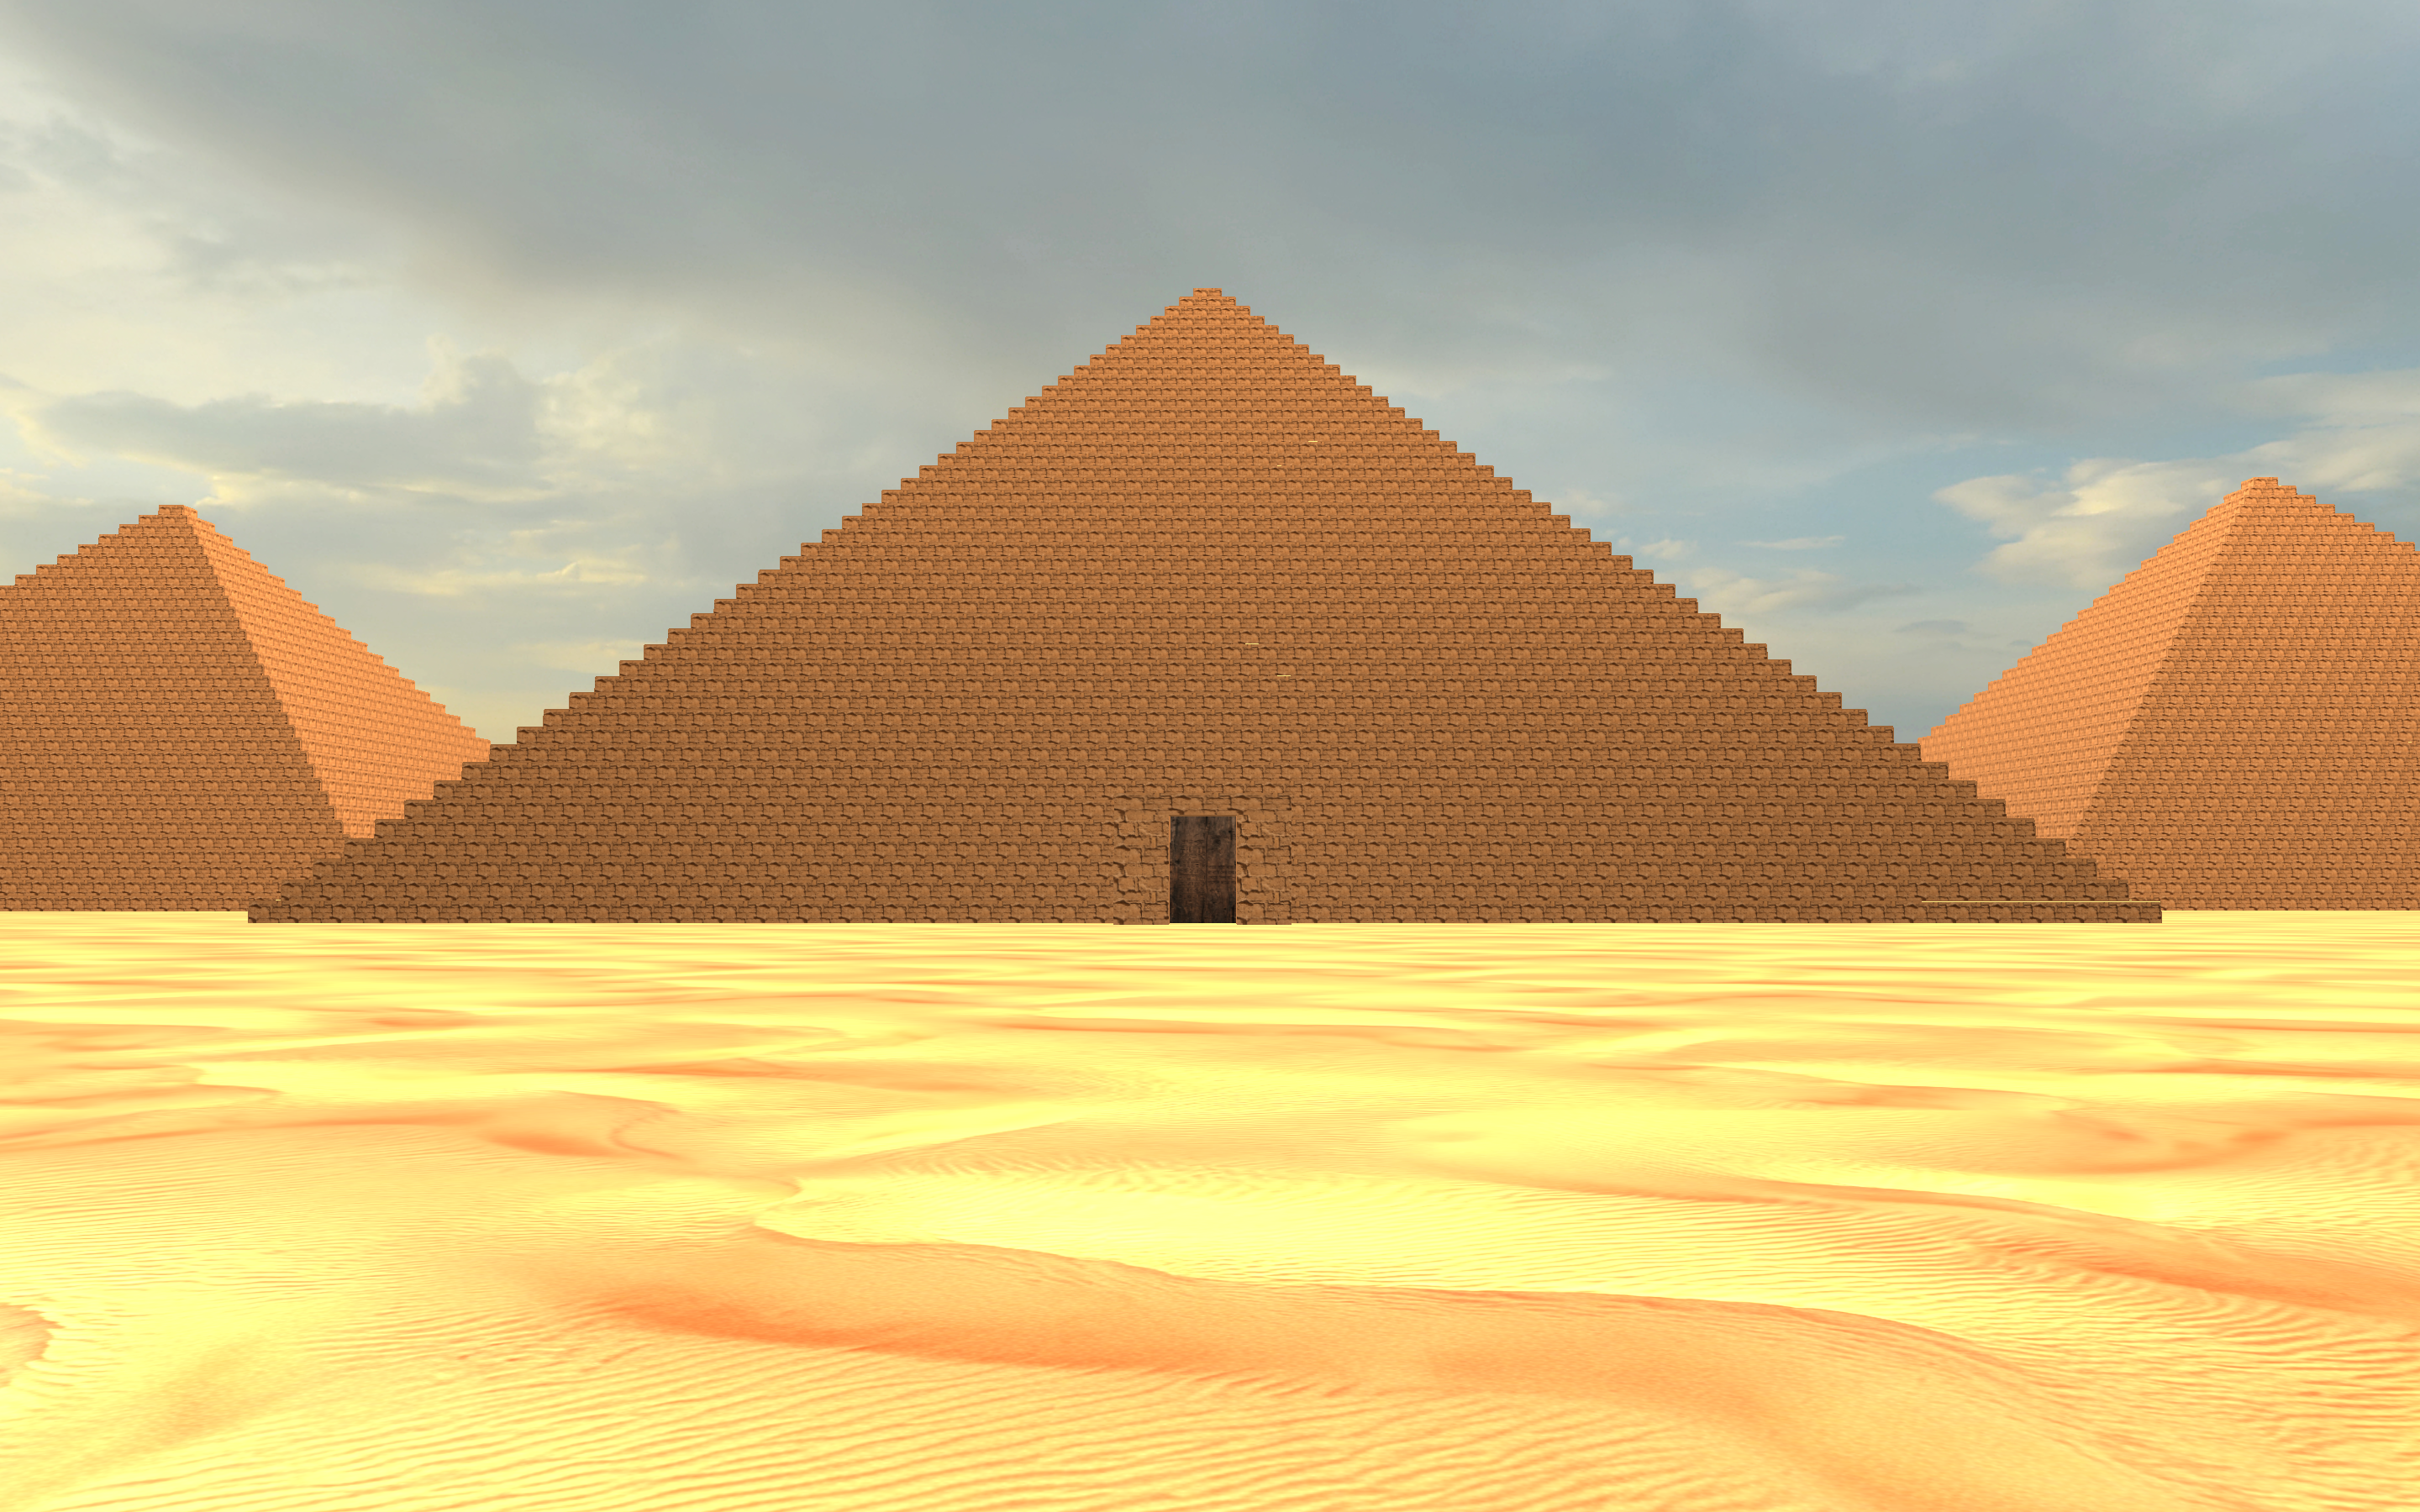
\includegraphics[width=0.9\textwidth]{screenshots/1.png}
    \caption{The foundational Pyramids rendered precisely applying procedural geometric primitives under global Directional Sunlight, demonstrating standard texturing implementations mapping standard ambient bounds uniformly across the desert terrain.}
    \label{fig:exterior_pyramids}
\end{figure}

\newpage

\begin{figure}[H]
    \centering
    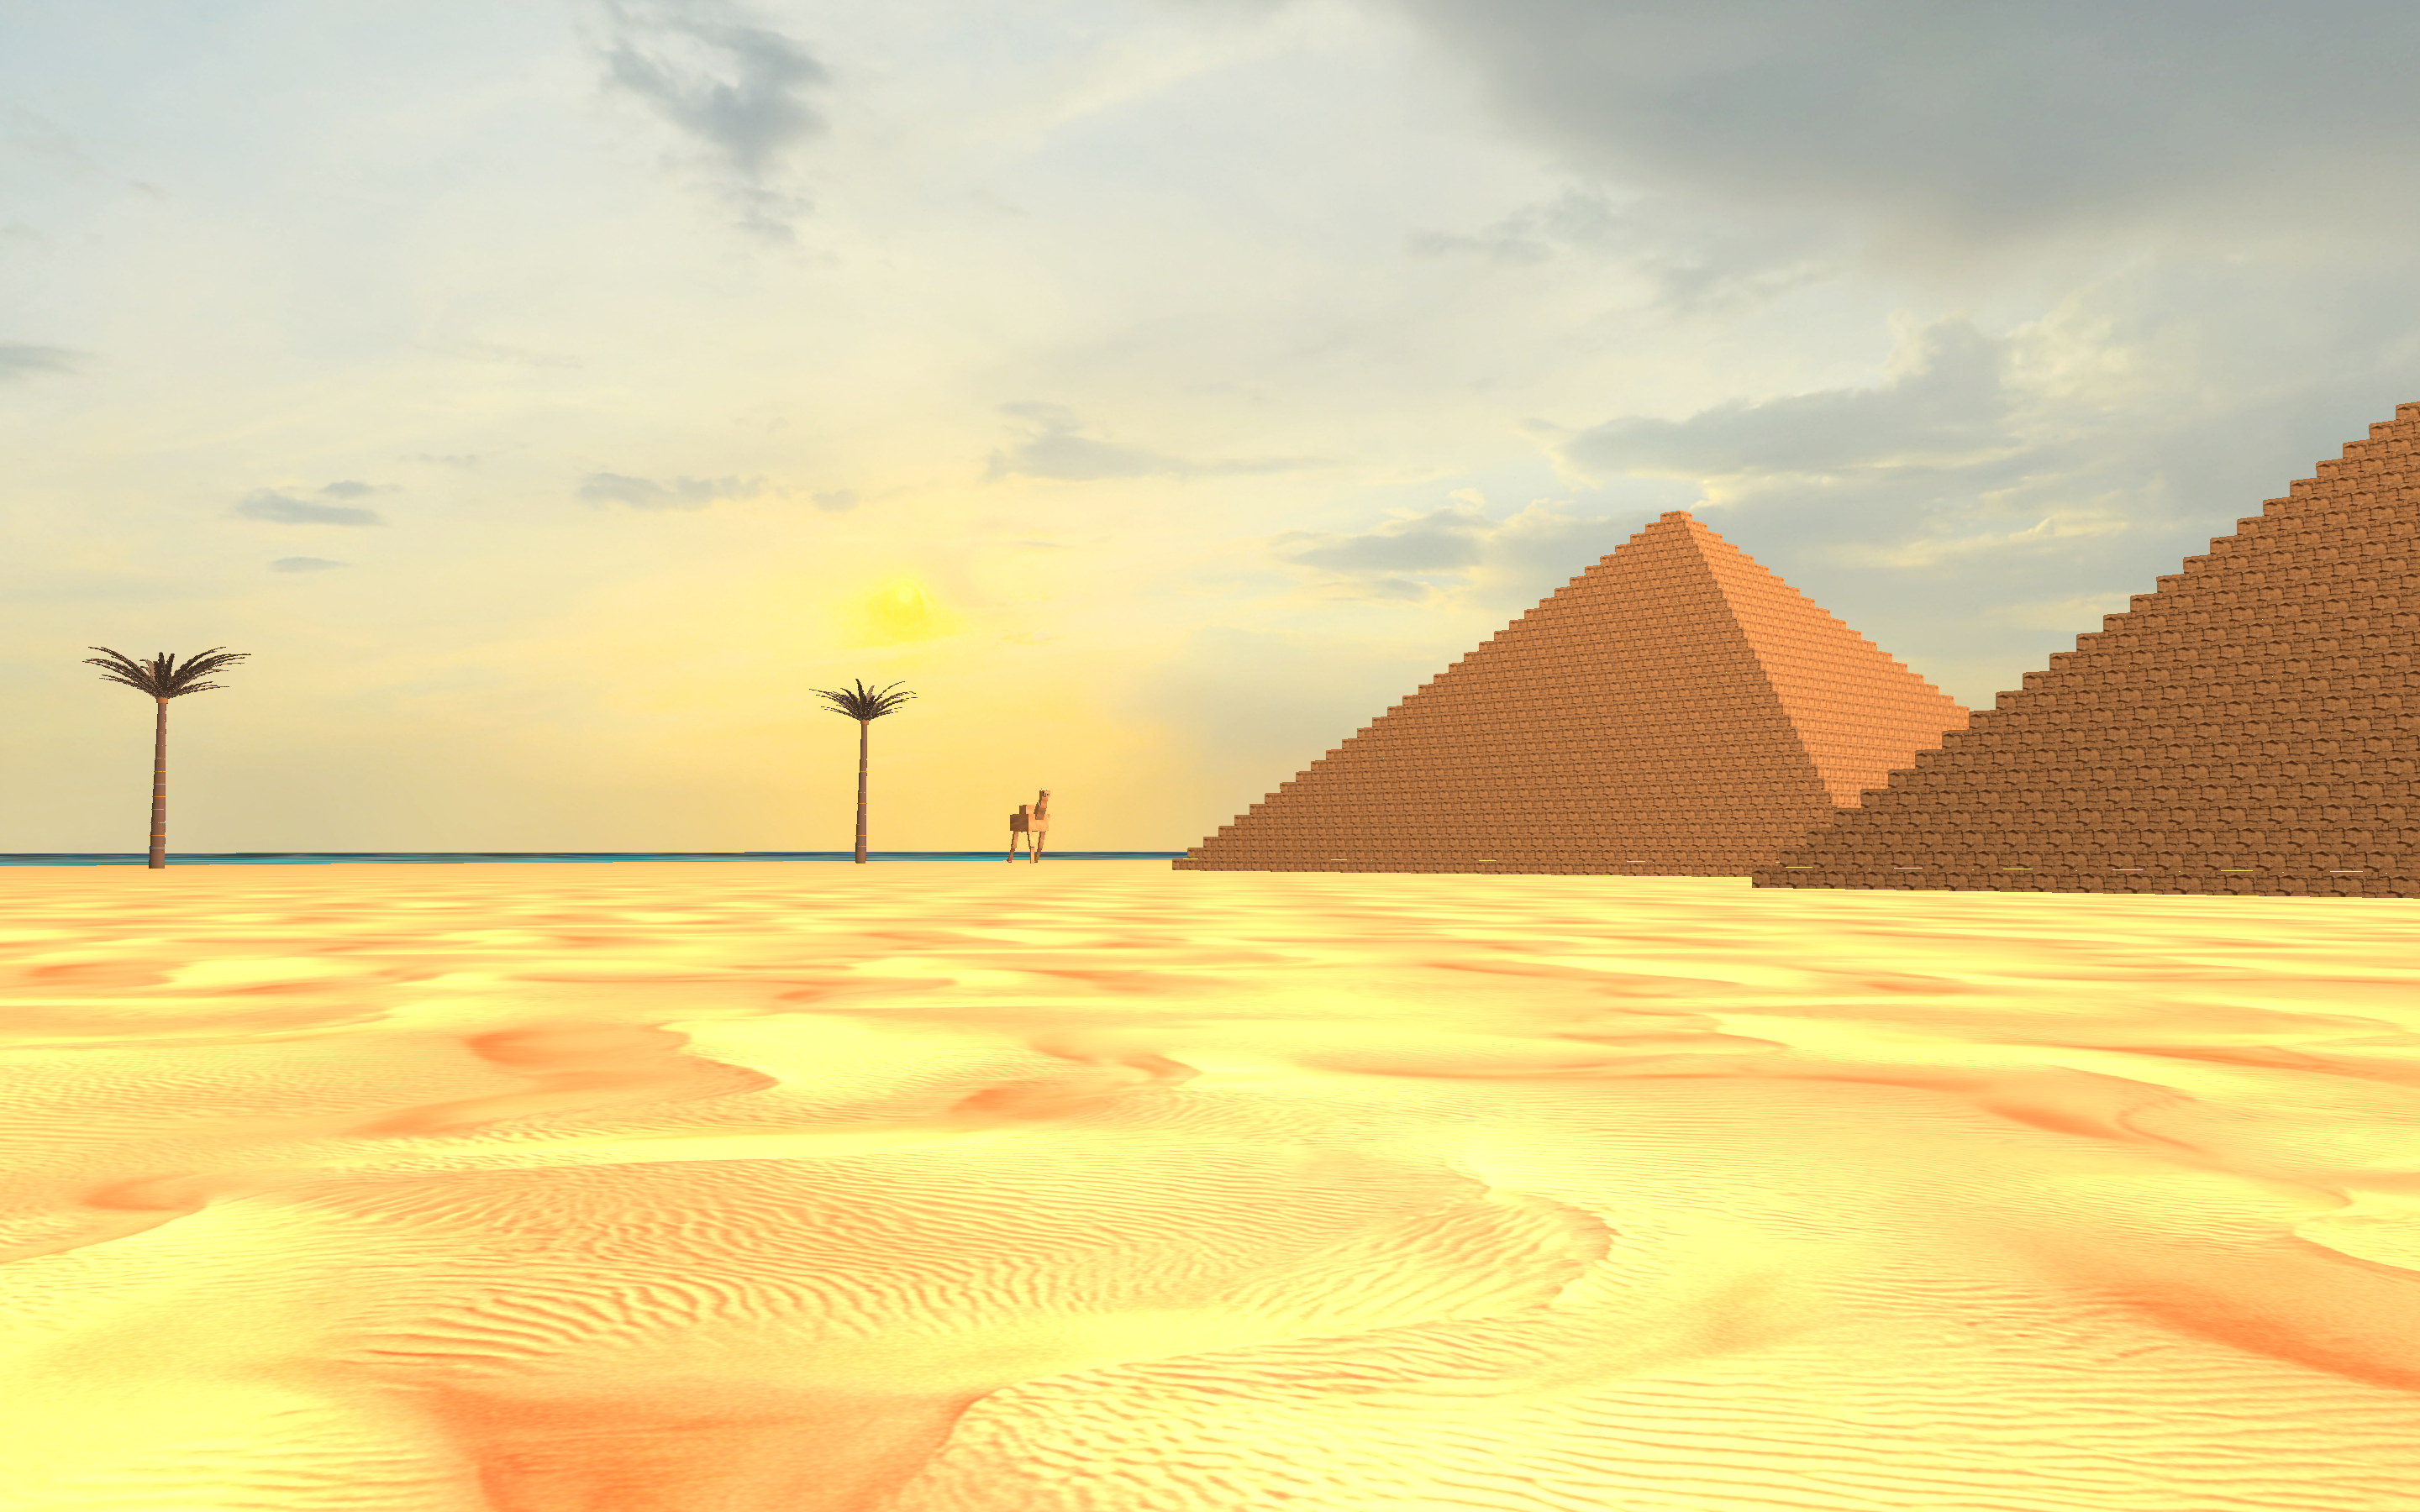
\includegraphics[width=0.9\textwidth]{screenshots/2.png}
    \caption{A wider exterior parameter illustrating hierarchical asset distribution consisting of an asymmetrical palm tree, procedural dunes, and the primary pyramid scaling gracefully against the global sunset gradients matching ambient bounds.}
    \label{fig:distant_pyramids}
\end{figure}

\begin{figure}[H]
    \centering
    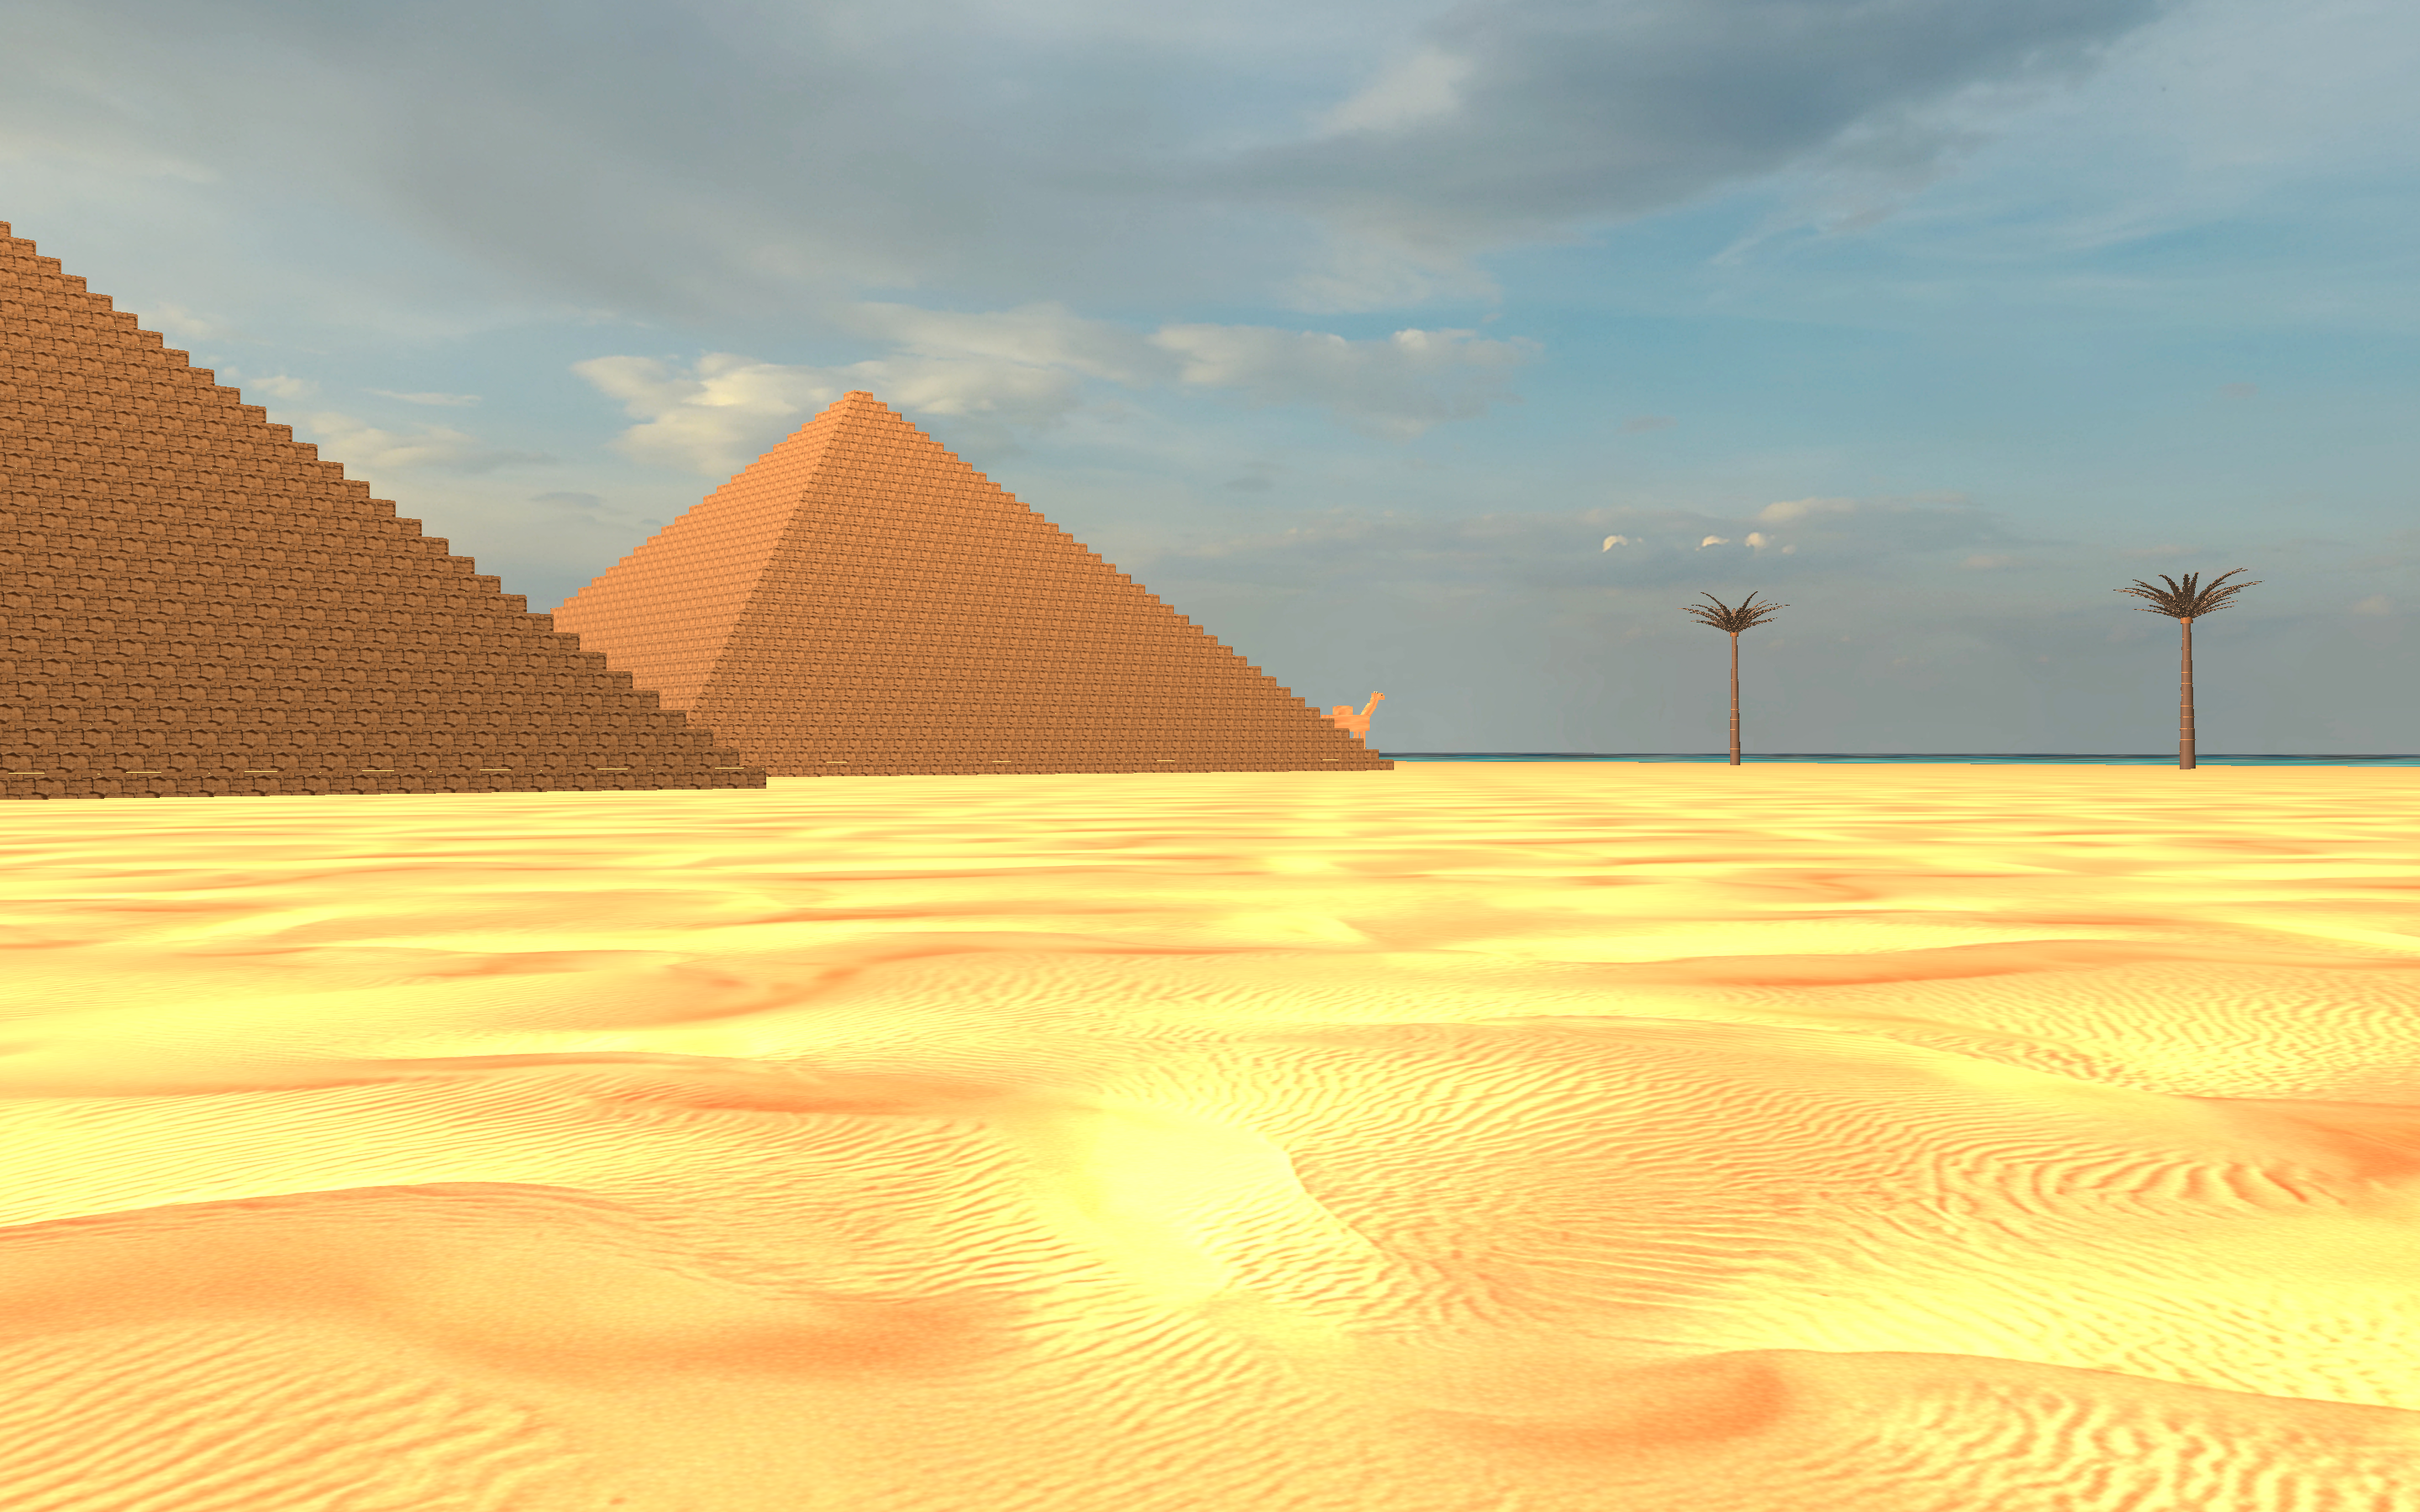
\includegraphics[width=0.9\textwidth]{screenshots/3.png}
    \caption{Displaying depth-tested object occlusion. A procedurally mapped Camel structure overlapping the distant ocean physics and scaling pyramids dynamically rendered seamlessly in the GPU rasterizer algorithm.}
    \label{fig:camel_pyramids}
\end{figure}

\newpage

\begin{figure}[H]
    \centering
    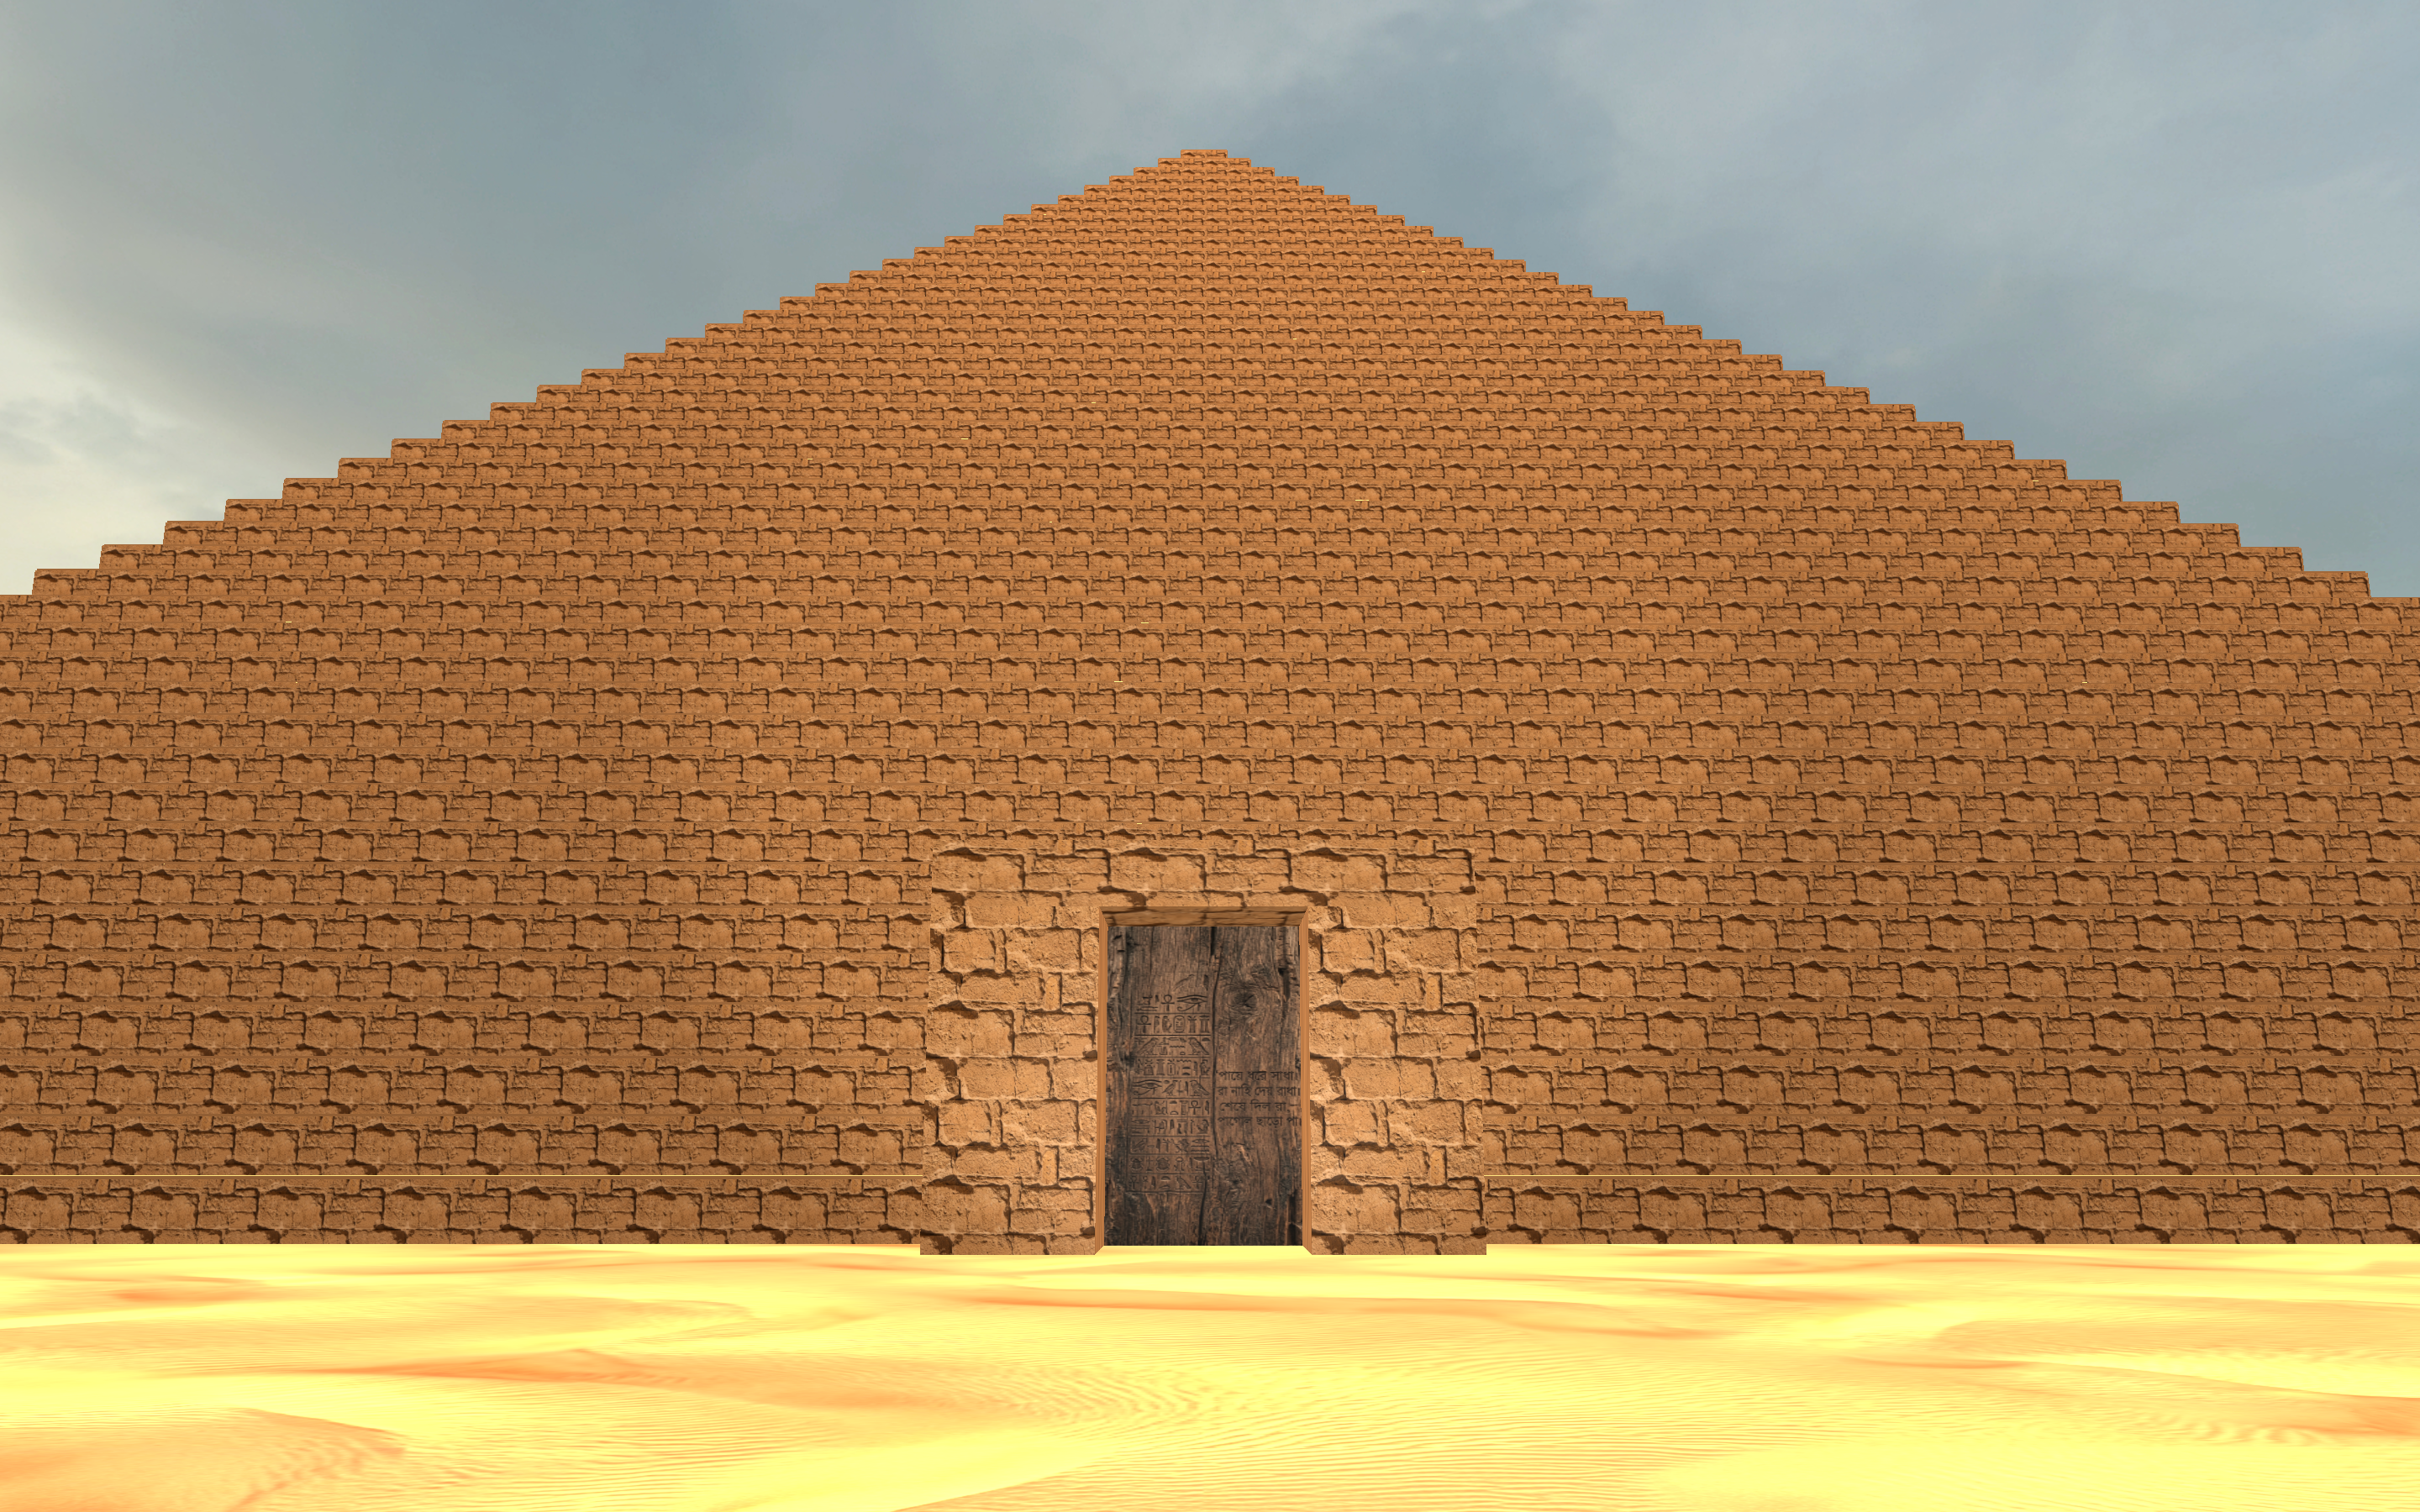
\includegraphics[width=0.9\textwidth]{screenshots/4.png}
    \caption{A distant desert topography mapped procedurally exhibiting linear texture blends mimicking soft wave patterns across shifting sands, gradually transitioning strictly to the active oceanic bodies extending to the mathematical horizon limits.}
    \label{fig:desert_view}
\end{figure}

\begin{figure}[H]
    \centering
    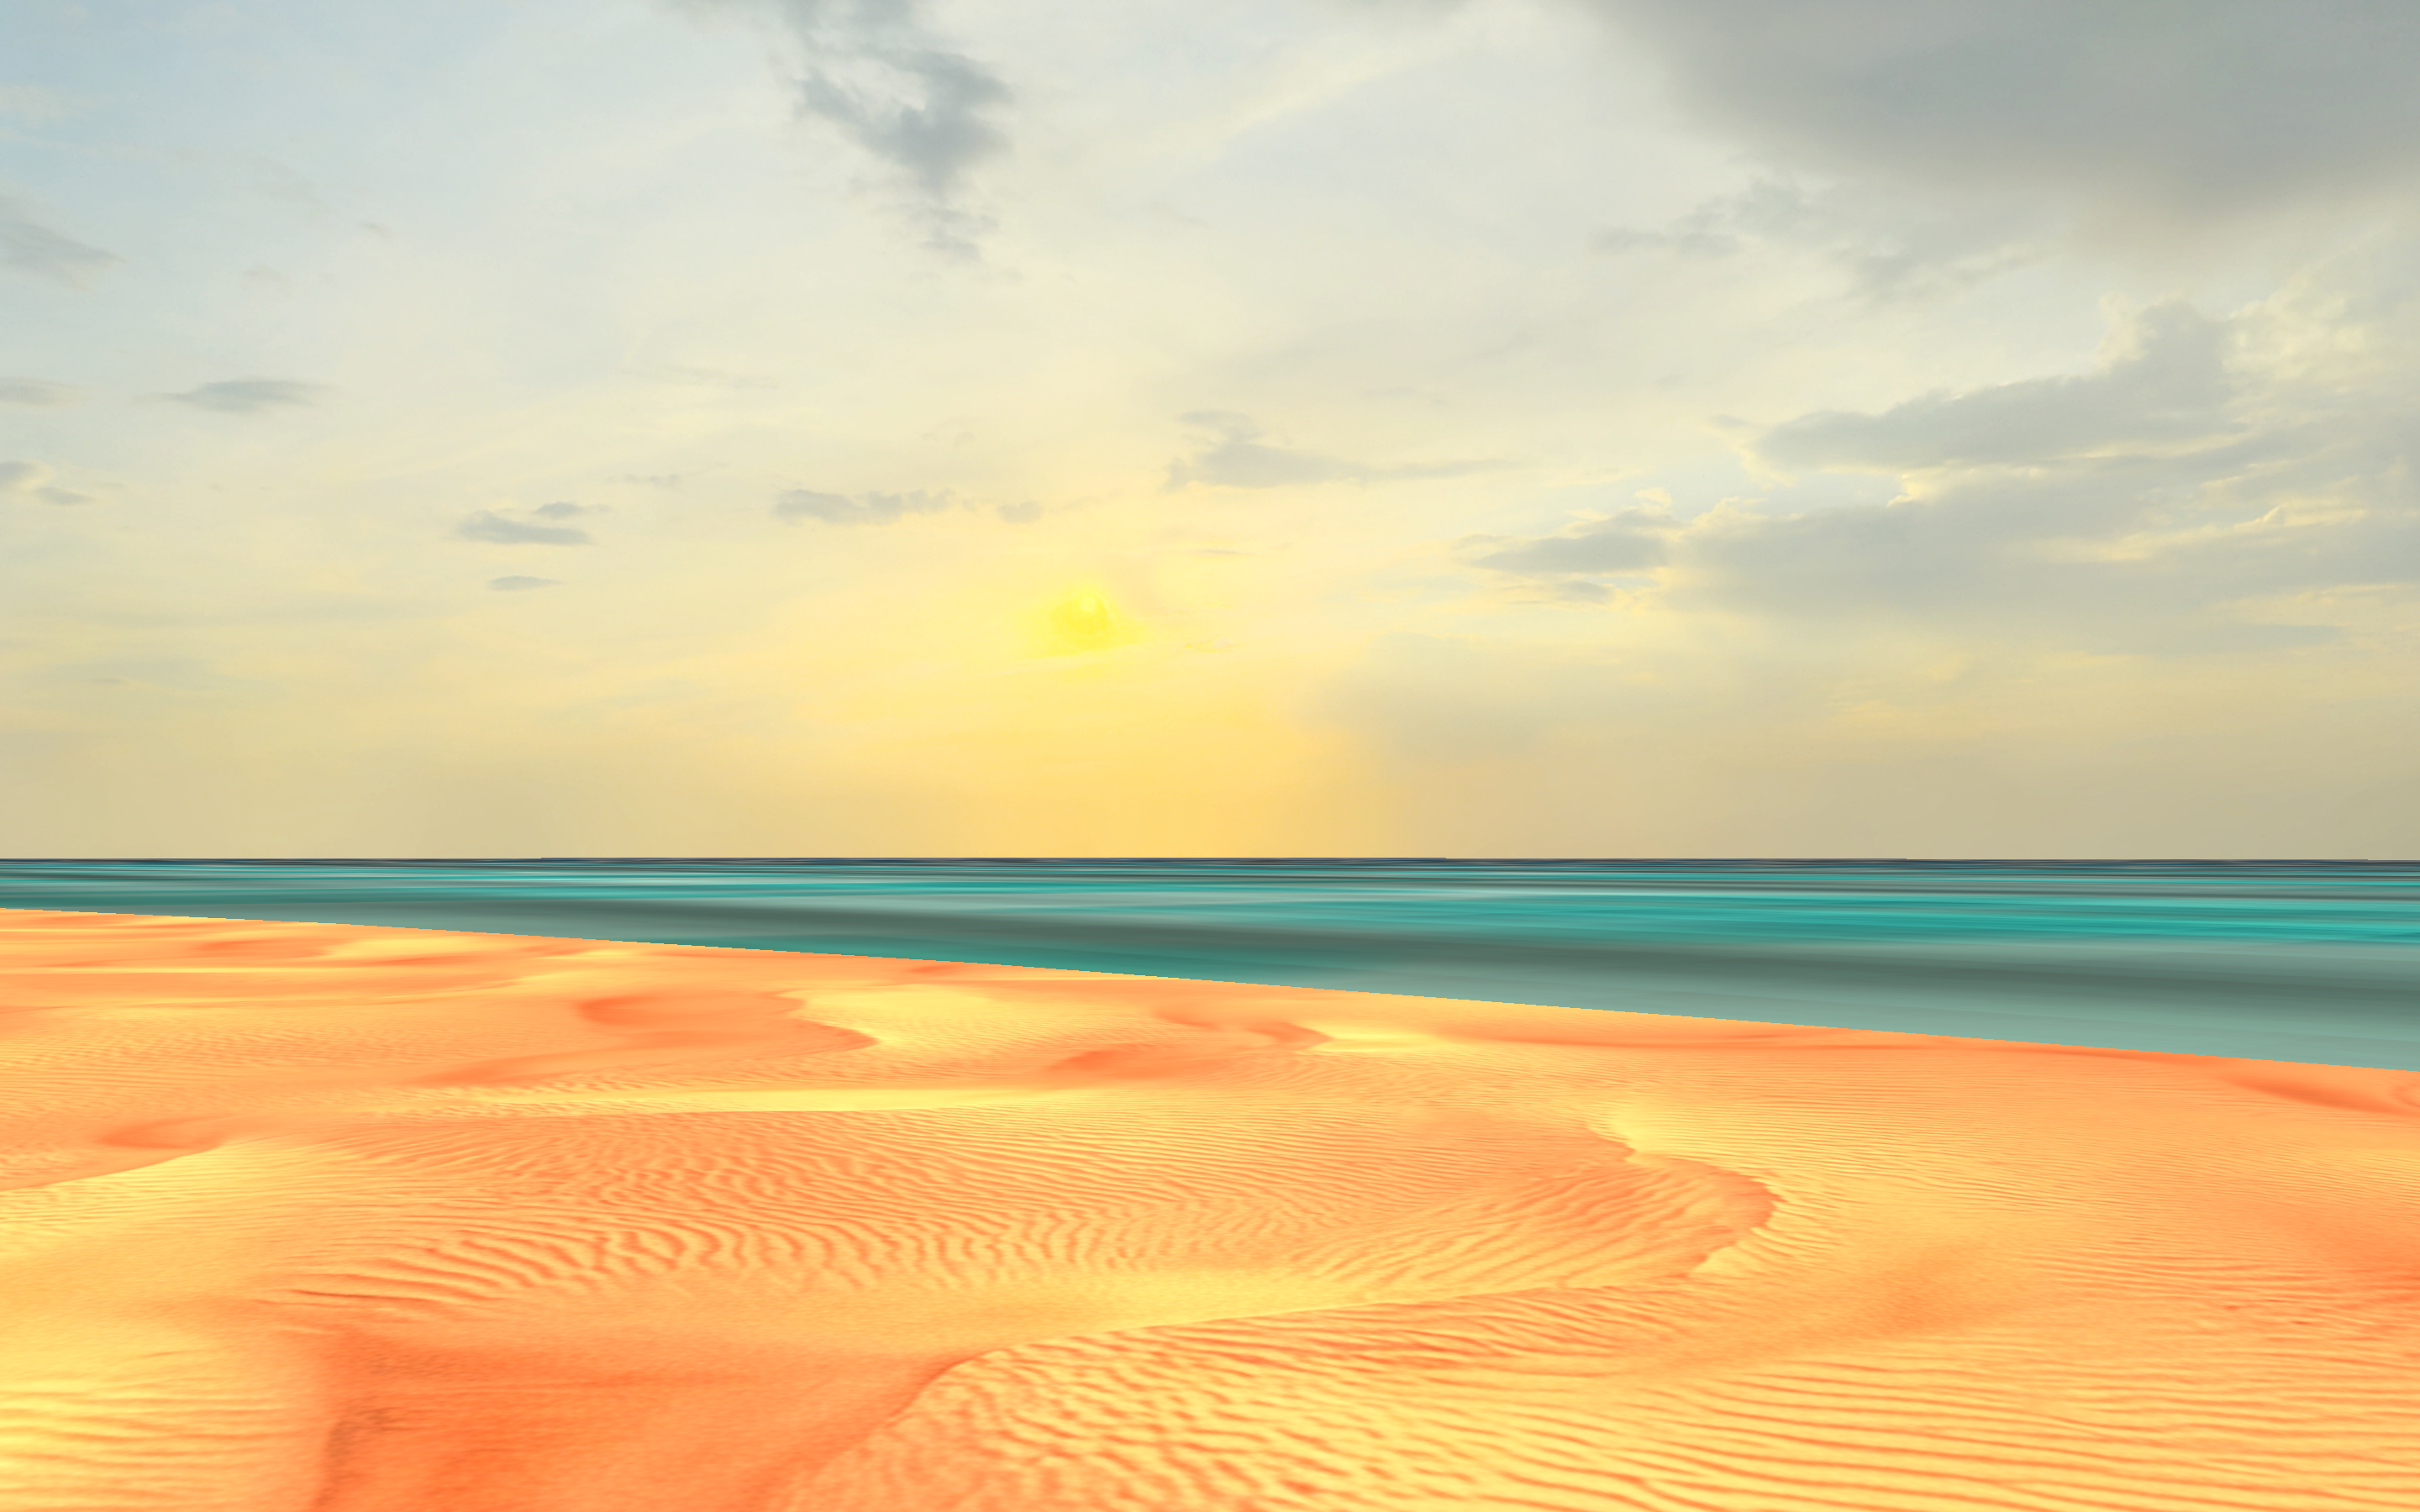
\includegraphics[width=0.9\textwidth]{screenshots/5.png}
    \caption{The implementation of parametric Bezier Curves natively evaluated within \texttt{vshader.glsl}, producing structural ocean wave displacements. The procedural fragment blending algorithms continuously mix bounds applying shallow depth colors transitioning into darker aquatic values dynamically representing volumetric absorption bounds.}
    \label{fig:ocean_bezier}
\end{figure}

\newpage

\begin{figure}[H]
    \centering
    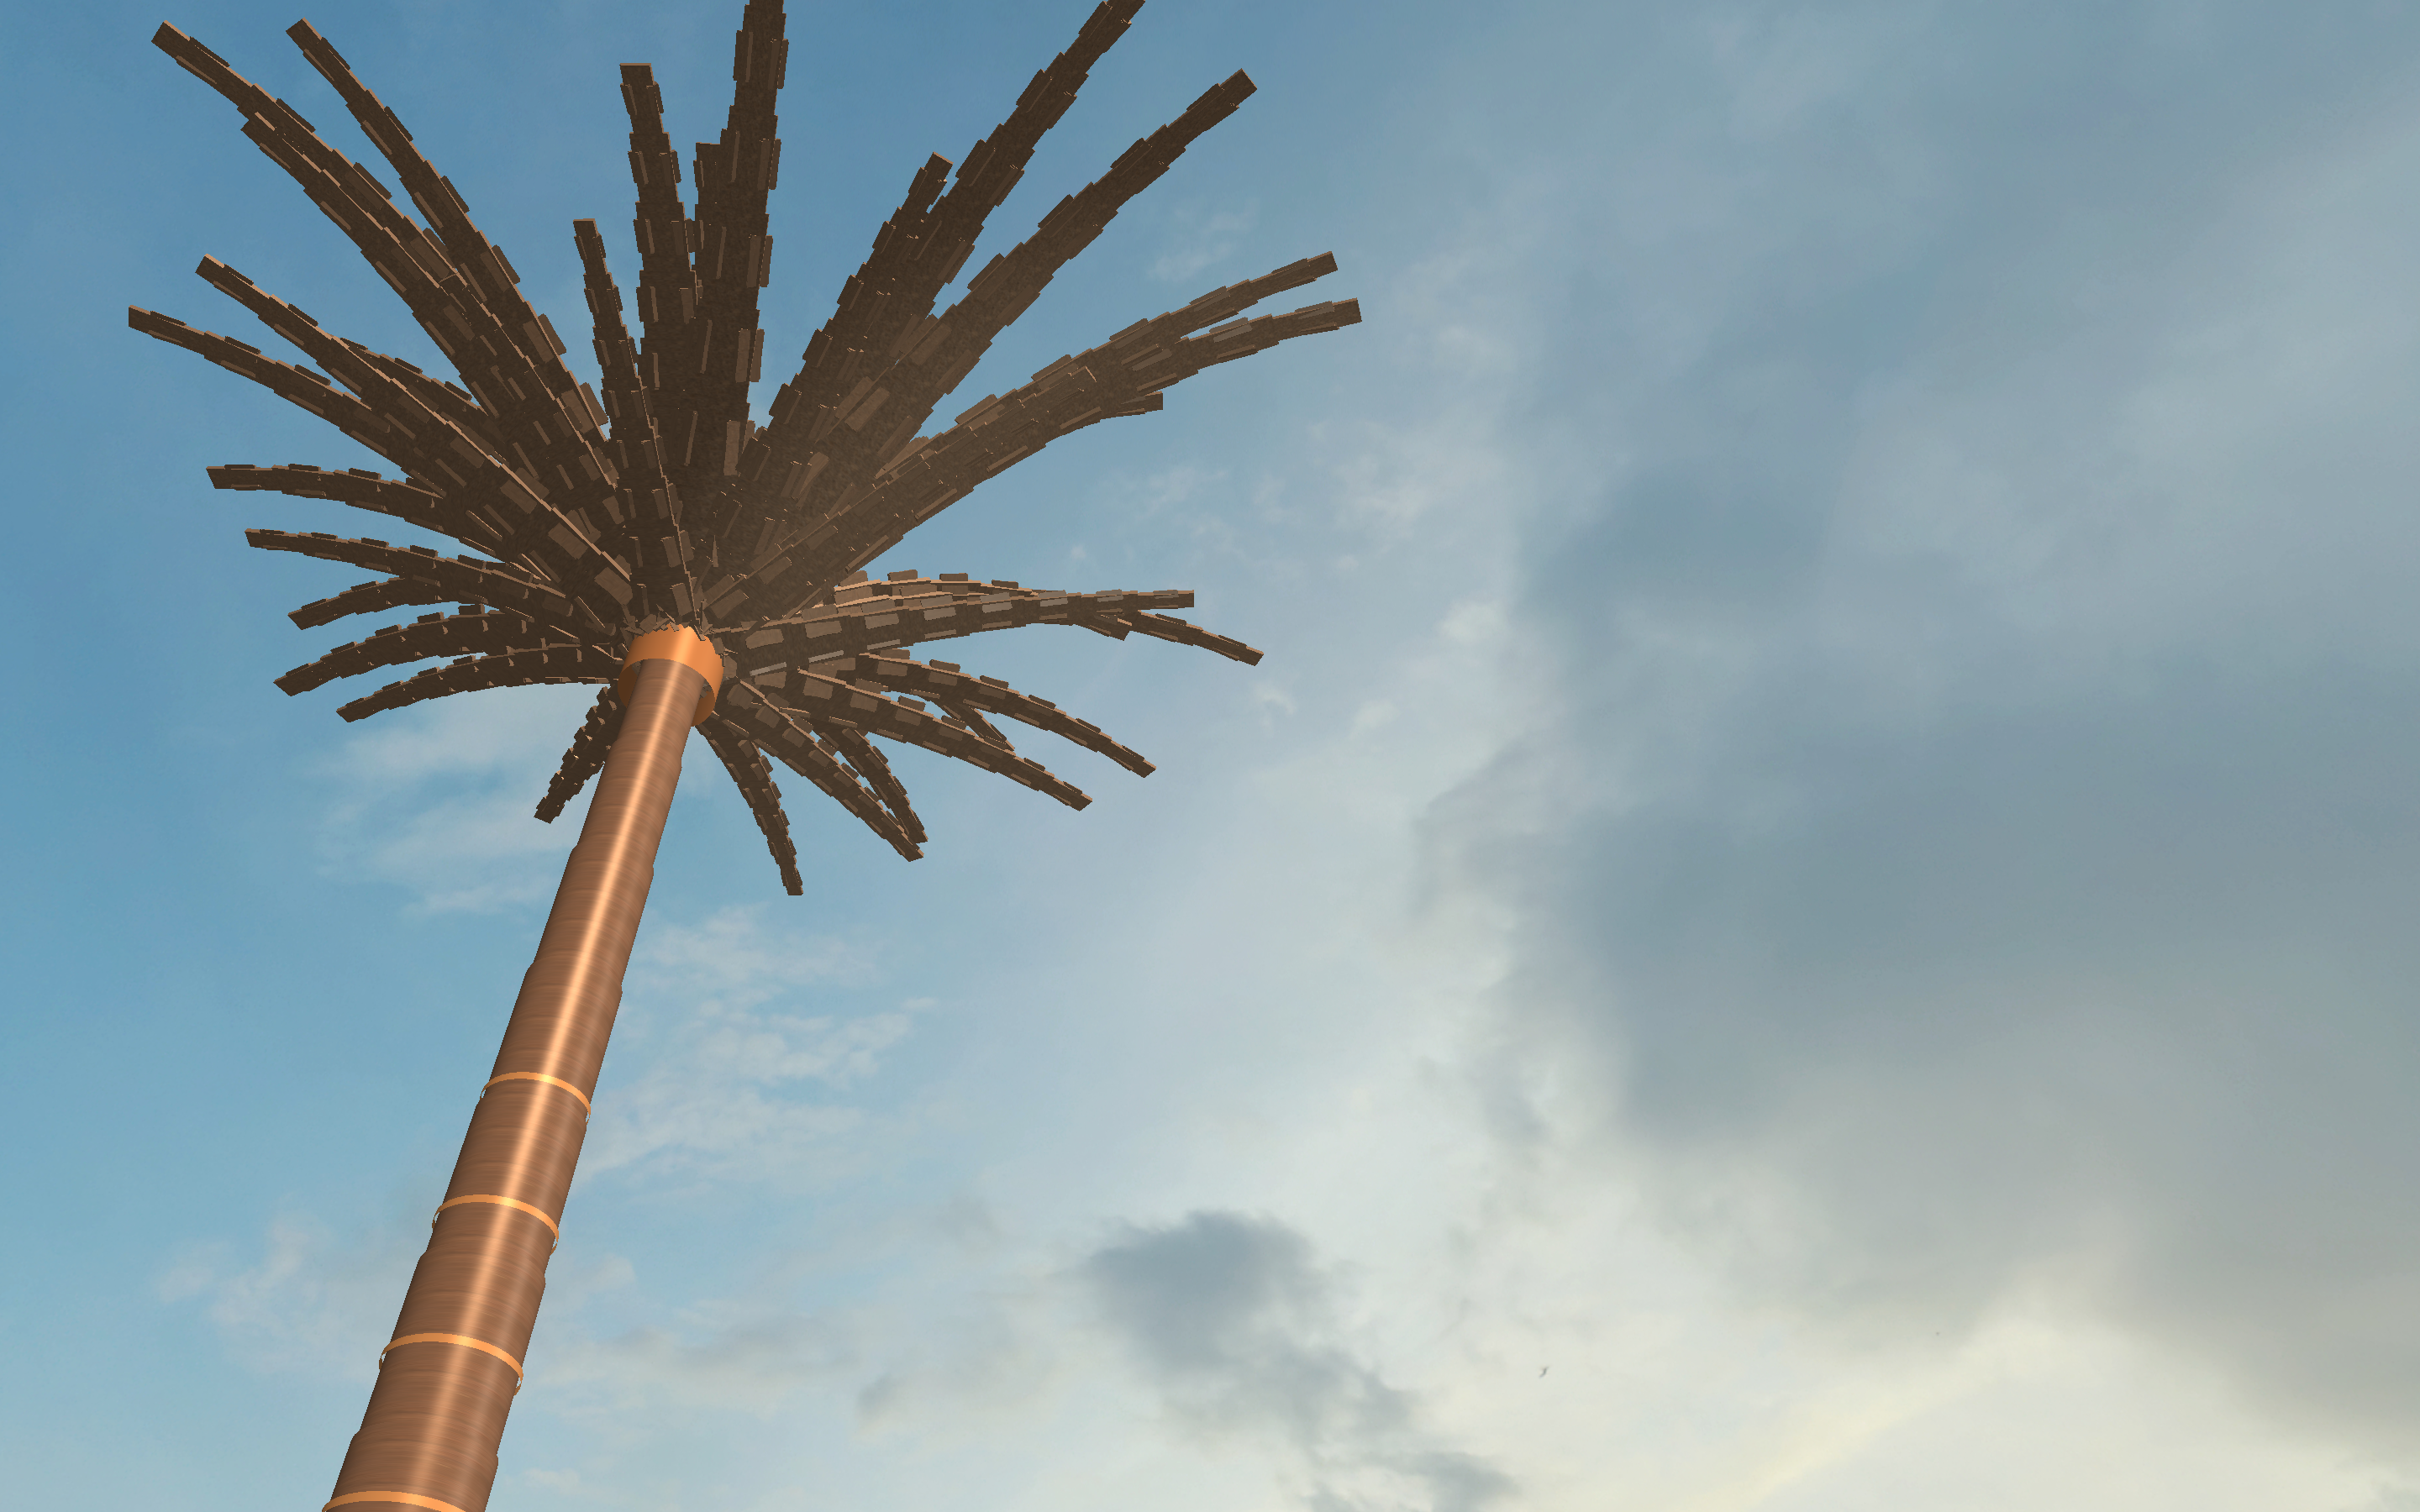
\includegraphics[width=0.9\textwidth]{screenshots/6.png}
    \caption{An intricate close-up inspecting visually detailed Palm Tree foliage structures. The system dynamically executes recursive fractal algorithms scaling geometrical primitive meshes exponentially to naturally assemble organic branching patterns.}
    \label{fig:fractal_tree}
\end{figure}

\begin{figure}[H]
    \centering
    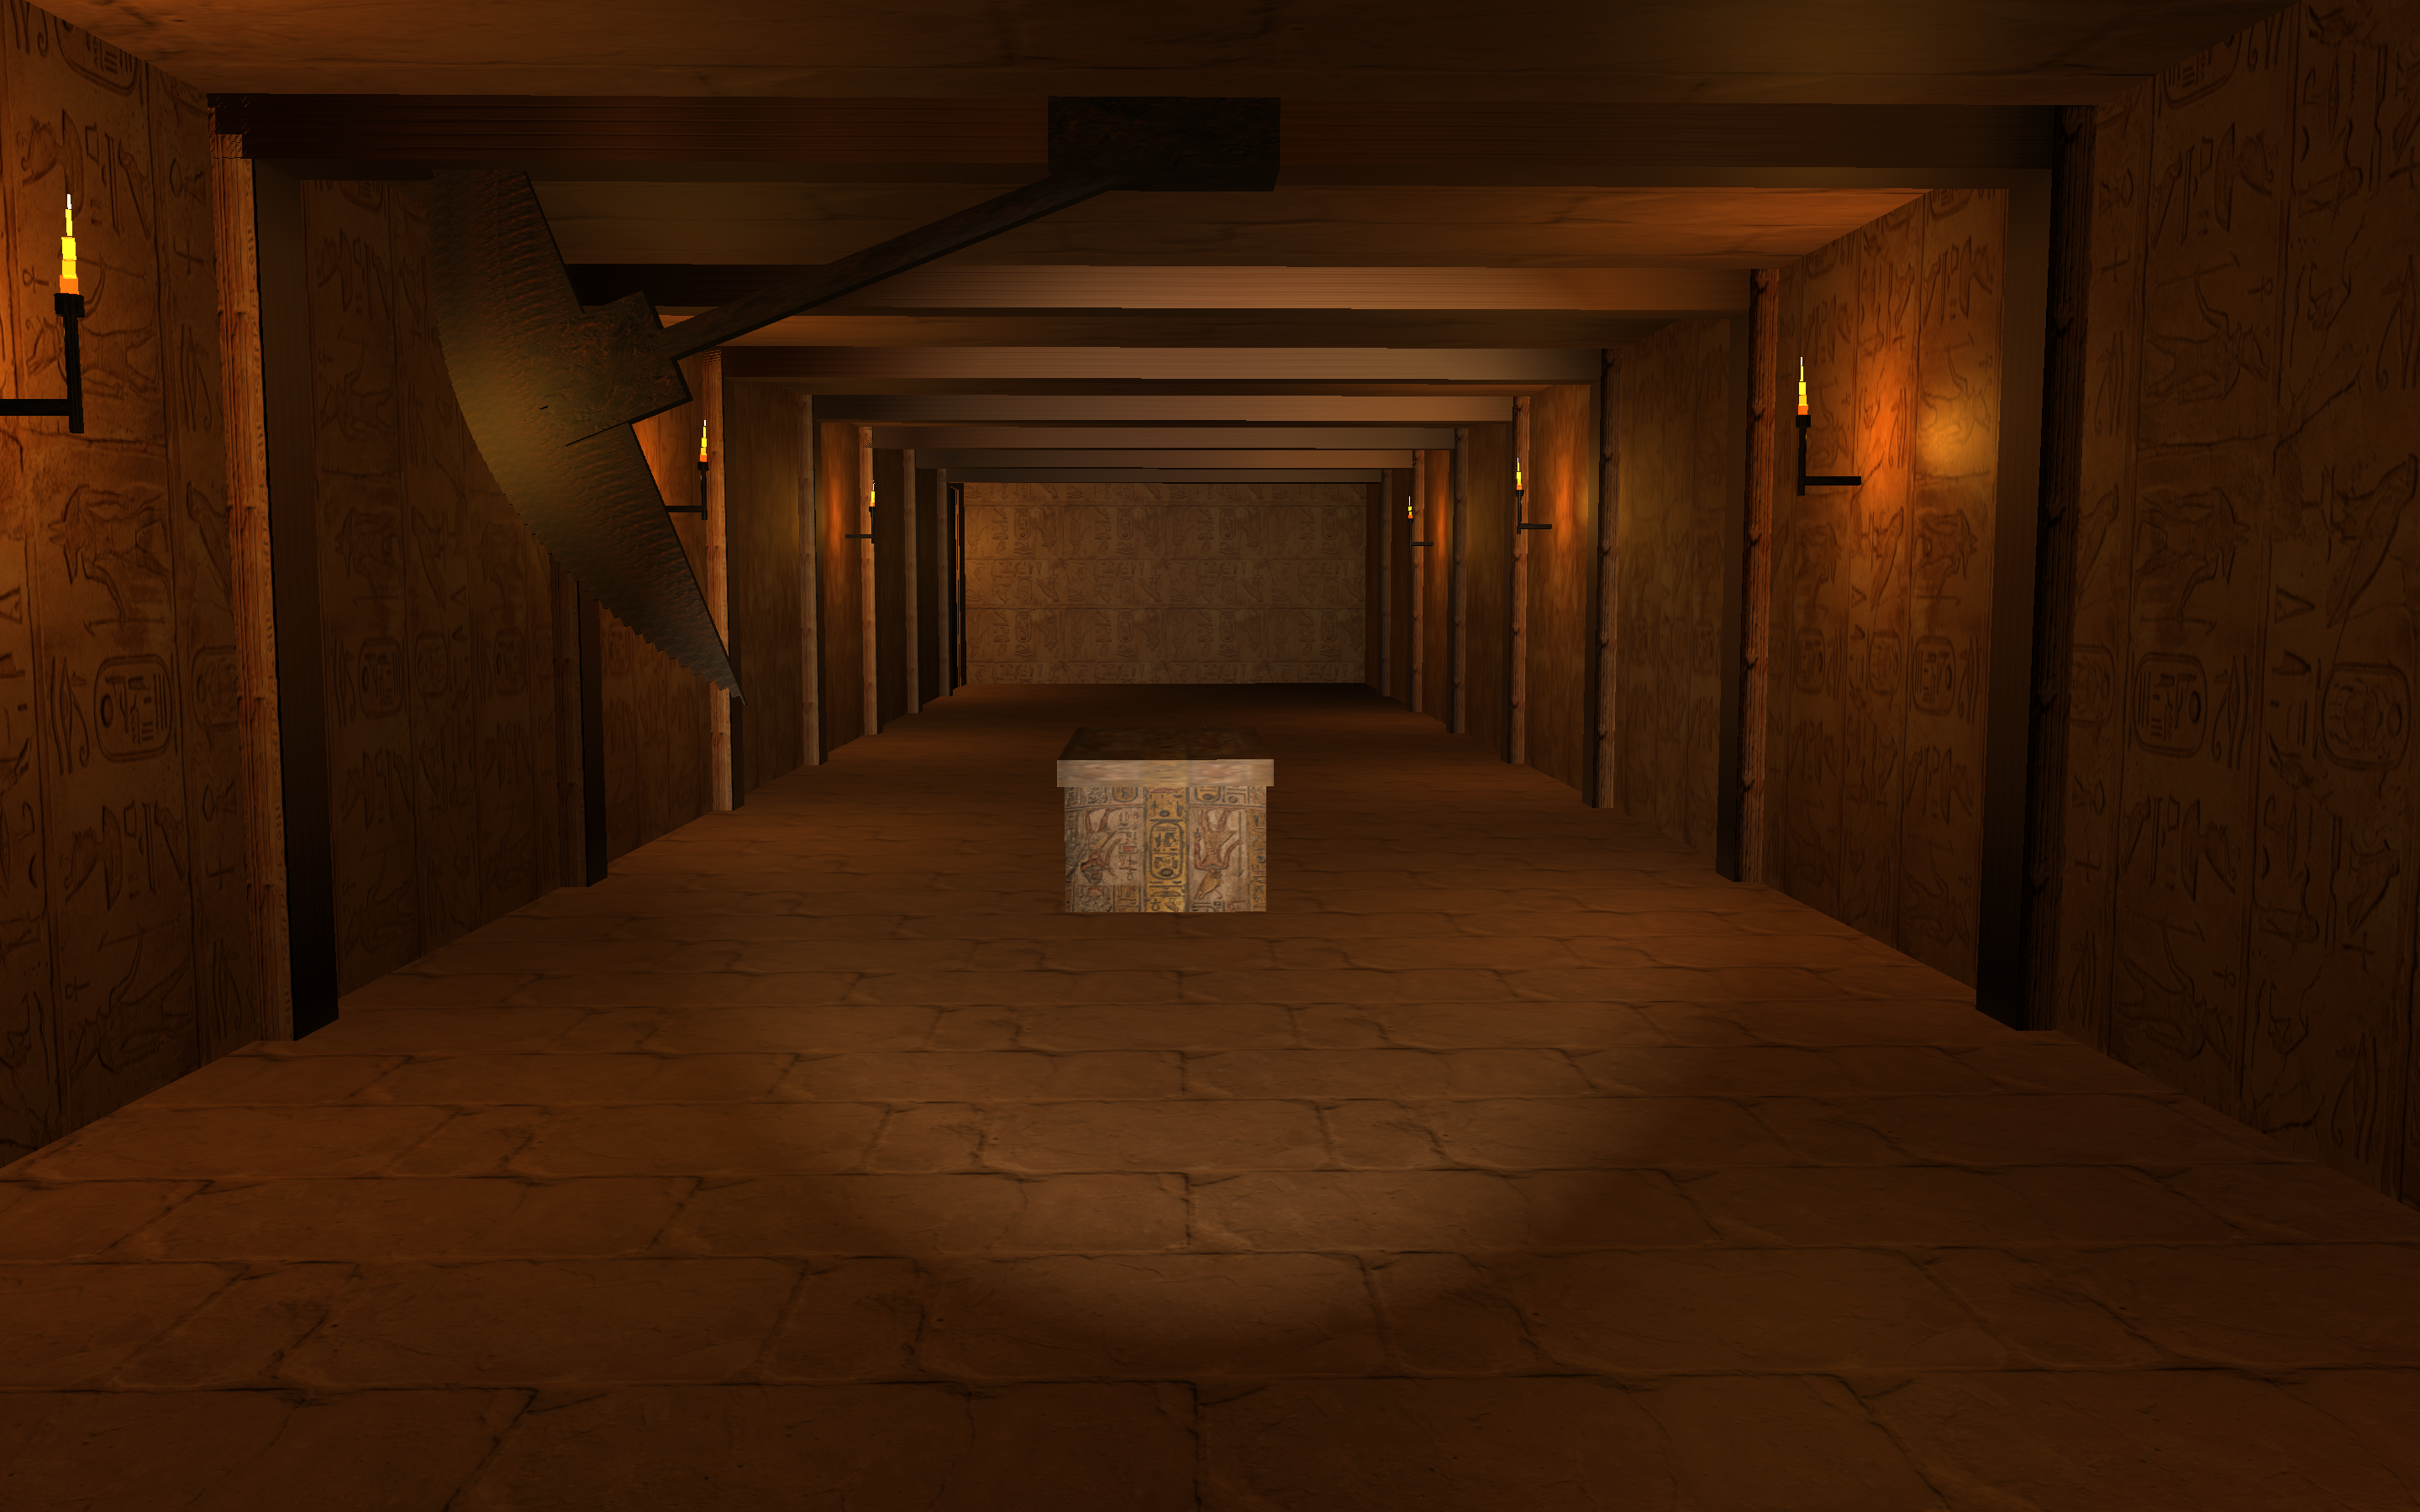
\includegraphics[width=0.9\textwidth]{screenshots/7.png}
    \caption{The primary underground T-shaped descending corridor, illuminated exclusively by Point Lights bound mathematically simulating lanterns. Showcases clear quadratic light attenuation smoothly dimming out traversing deeply into the architecture.}
    \label{fig:corridor_1}
\end{figure}

\newpage

\begin{figure}[H]
    \centering
    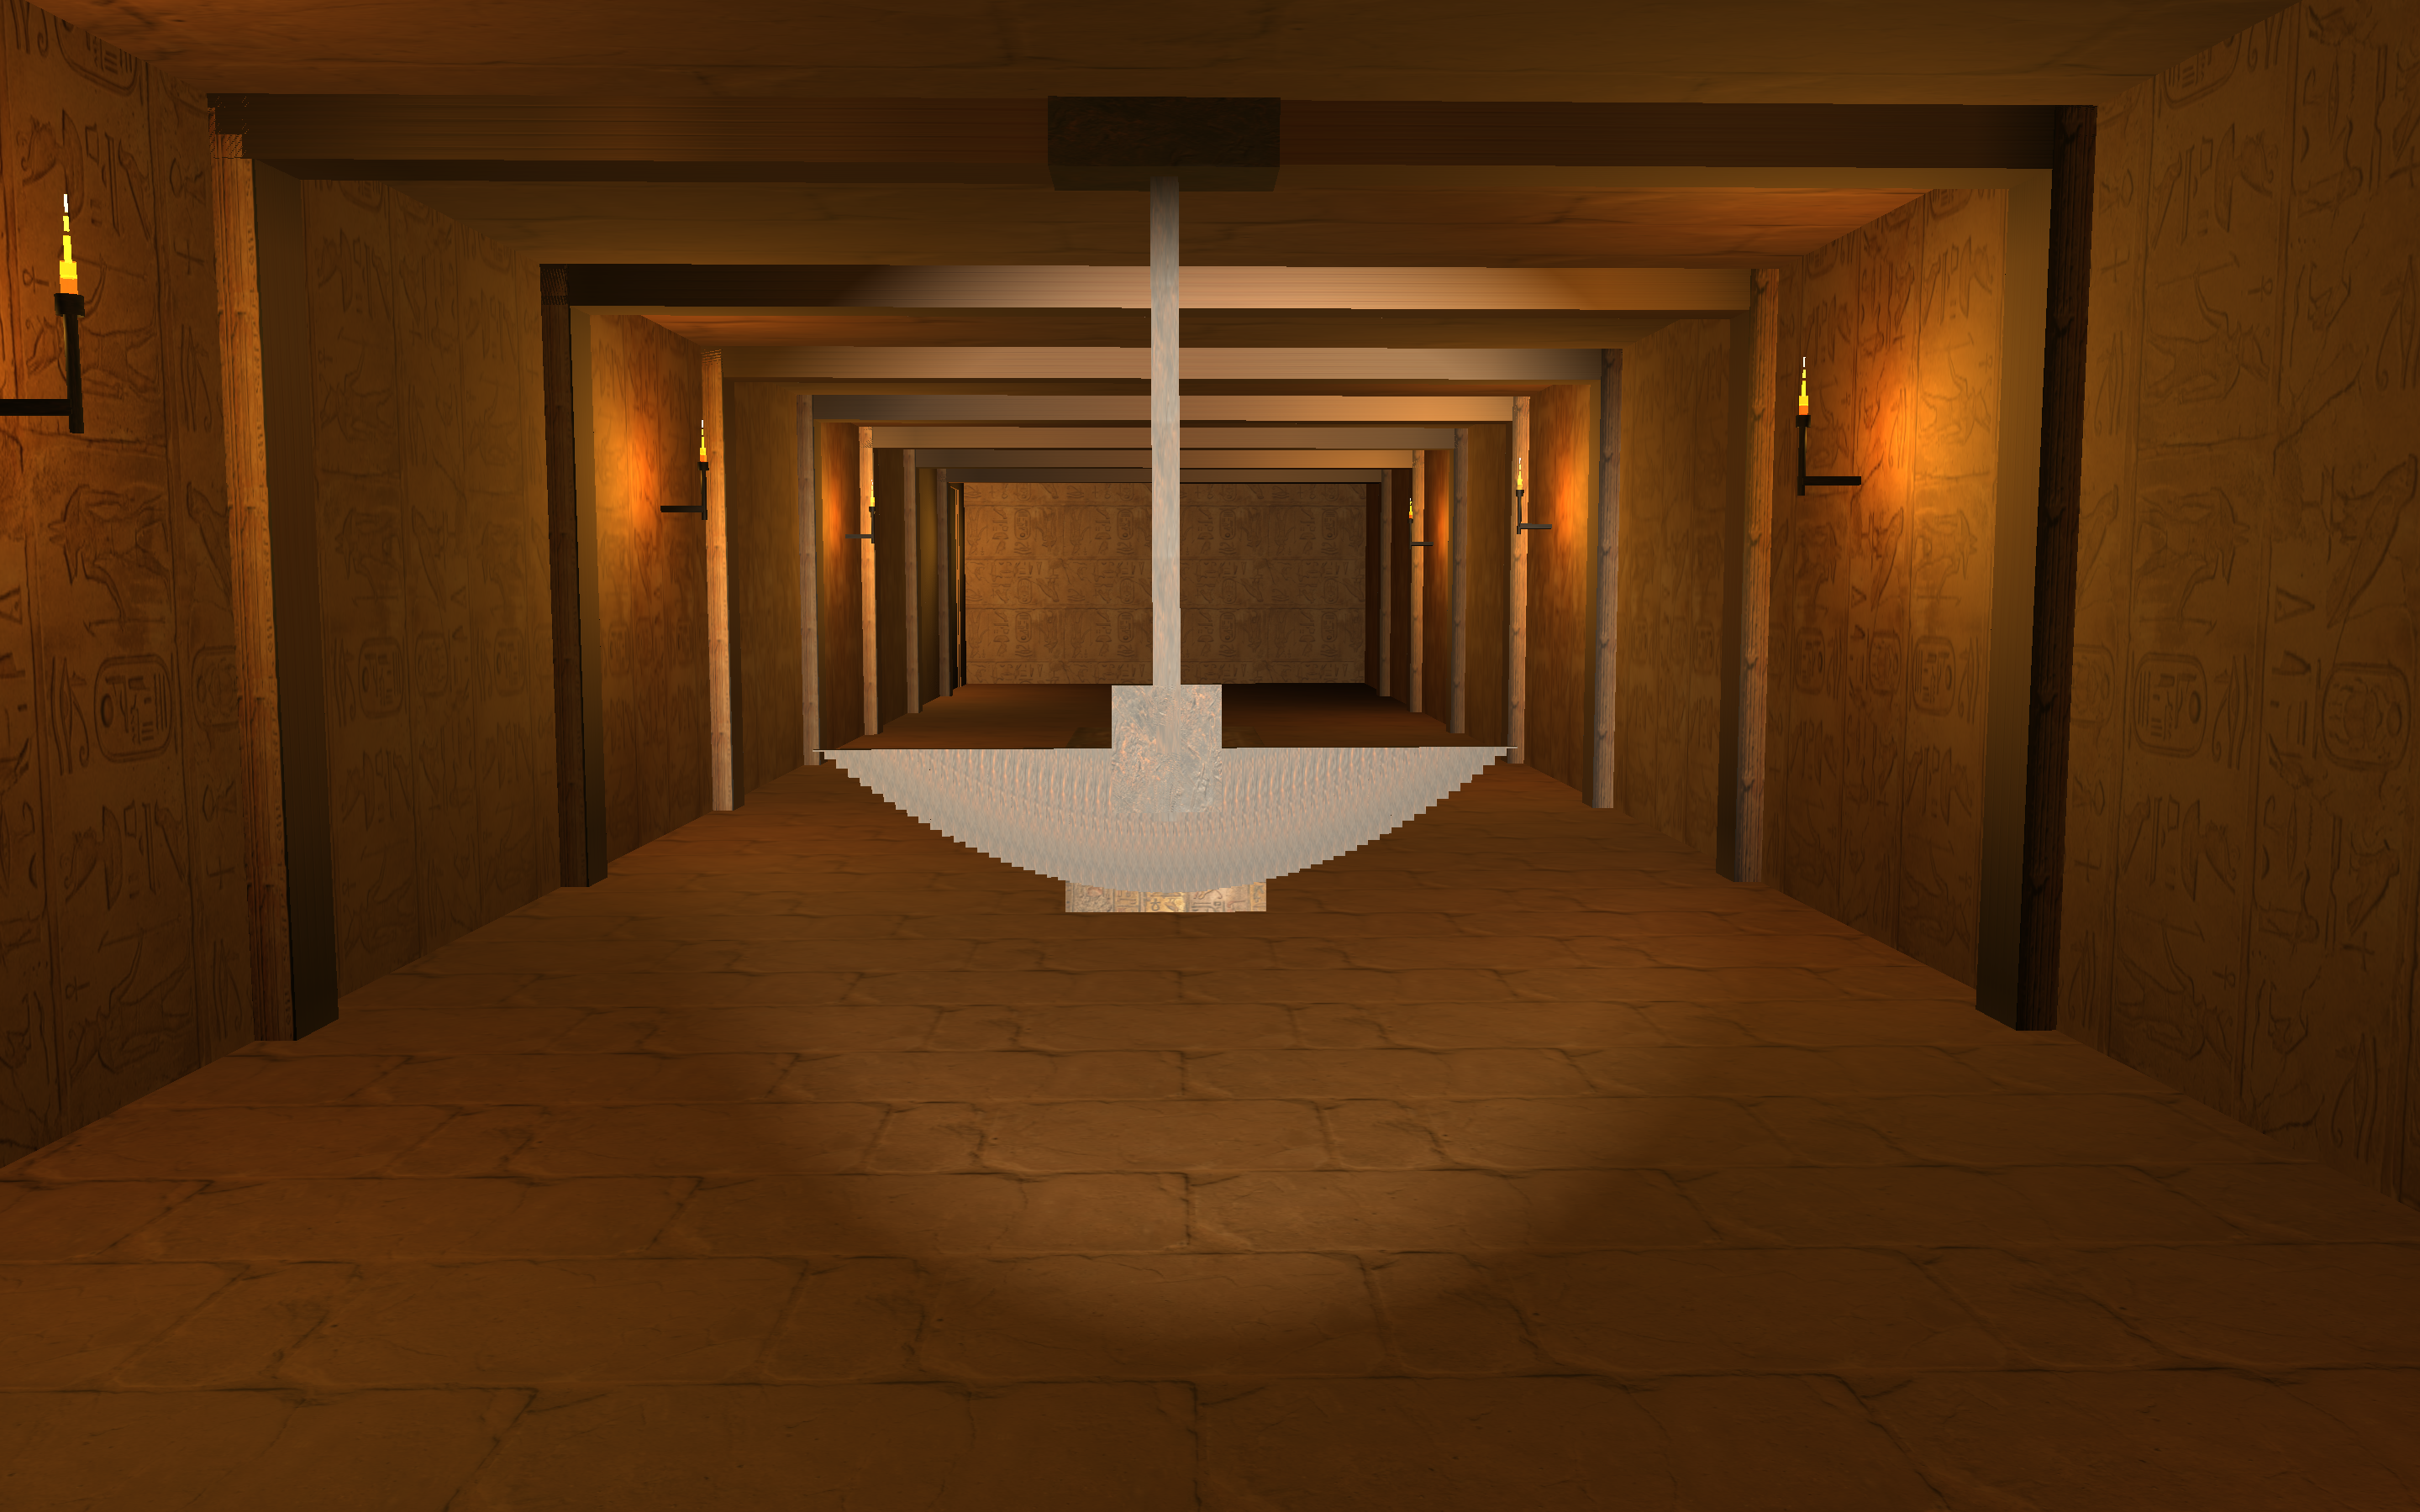
\includegraphics[width=0.9\textwidth]{screenshots/8.png}
    \caption{An alternate visualization of the identical descending corridor exhibiting fully maximized global ambient shader lighting without restrictive fragment loss tracking, utilized mainly for structural debugging.}
    \label{fig:corridor_full_ambient}
\end{figure}

\begin{figure}[H]
    \centering
    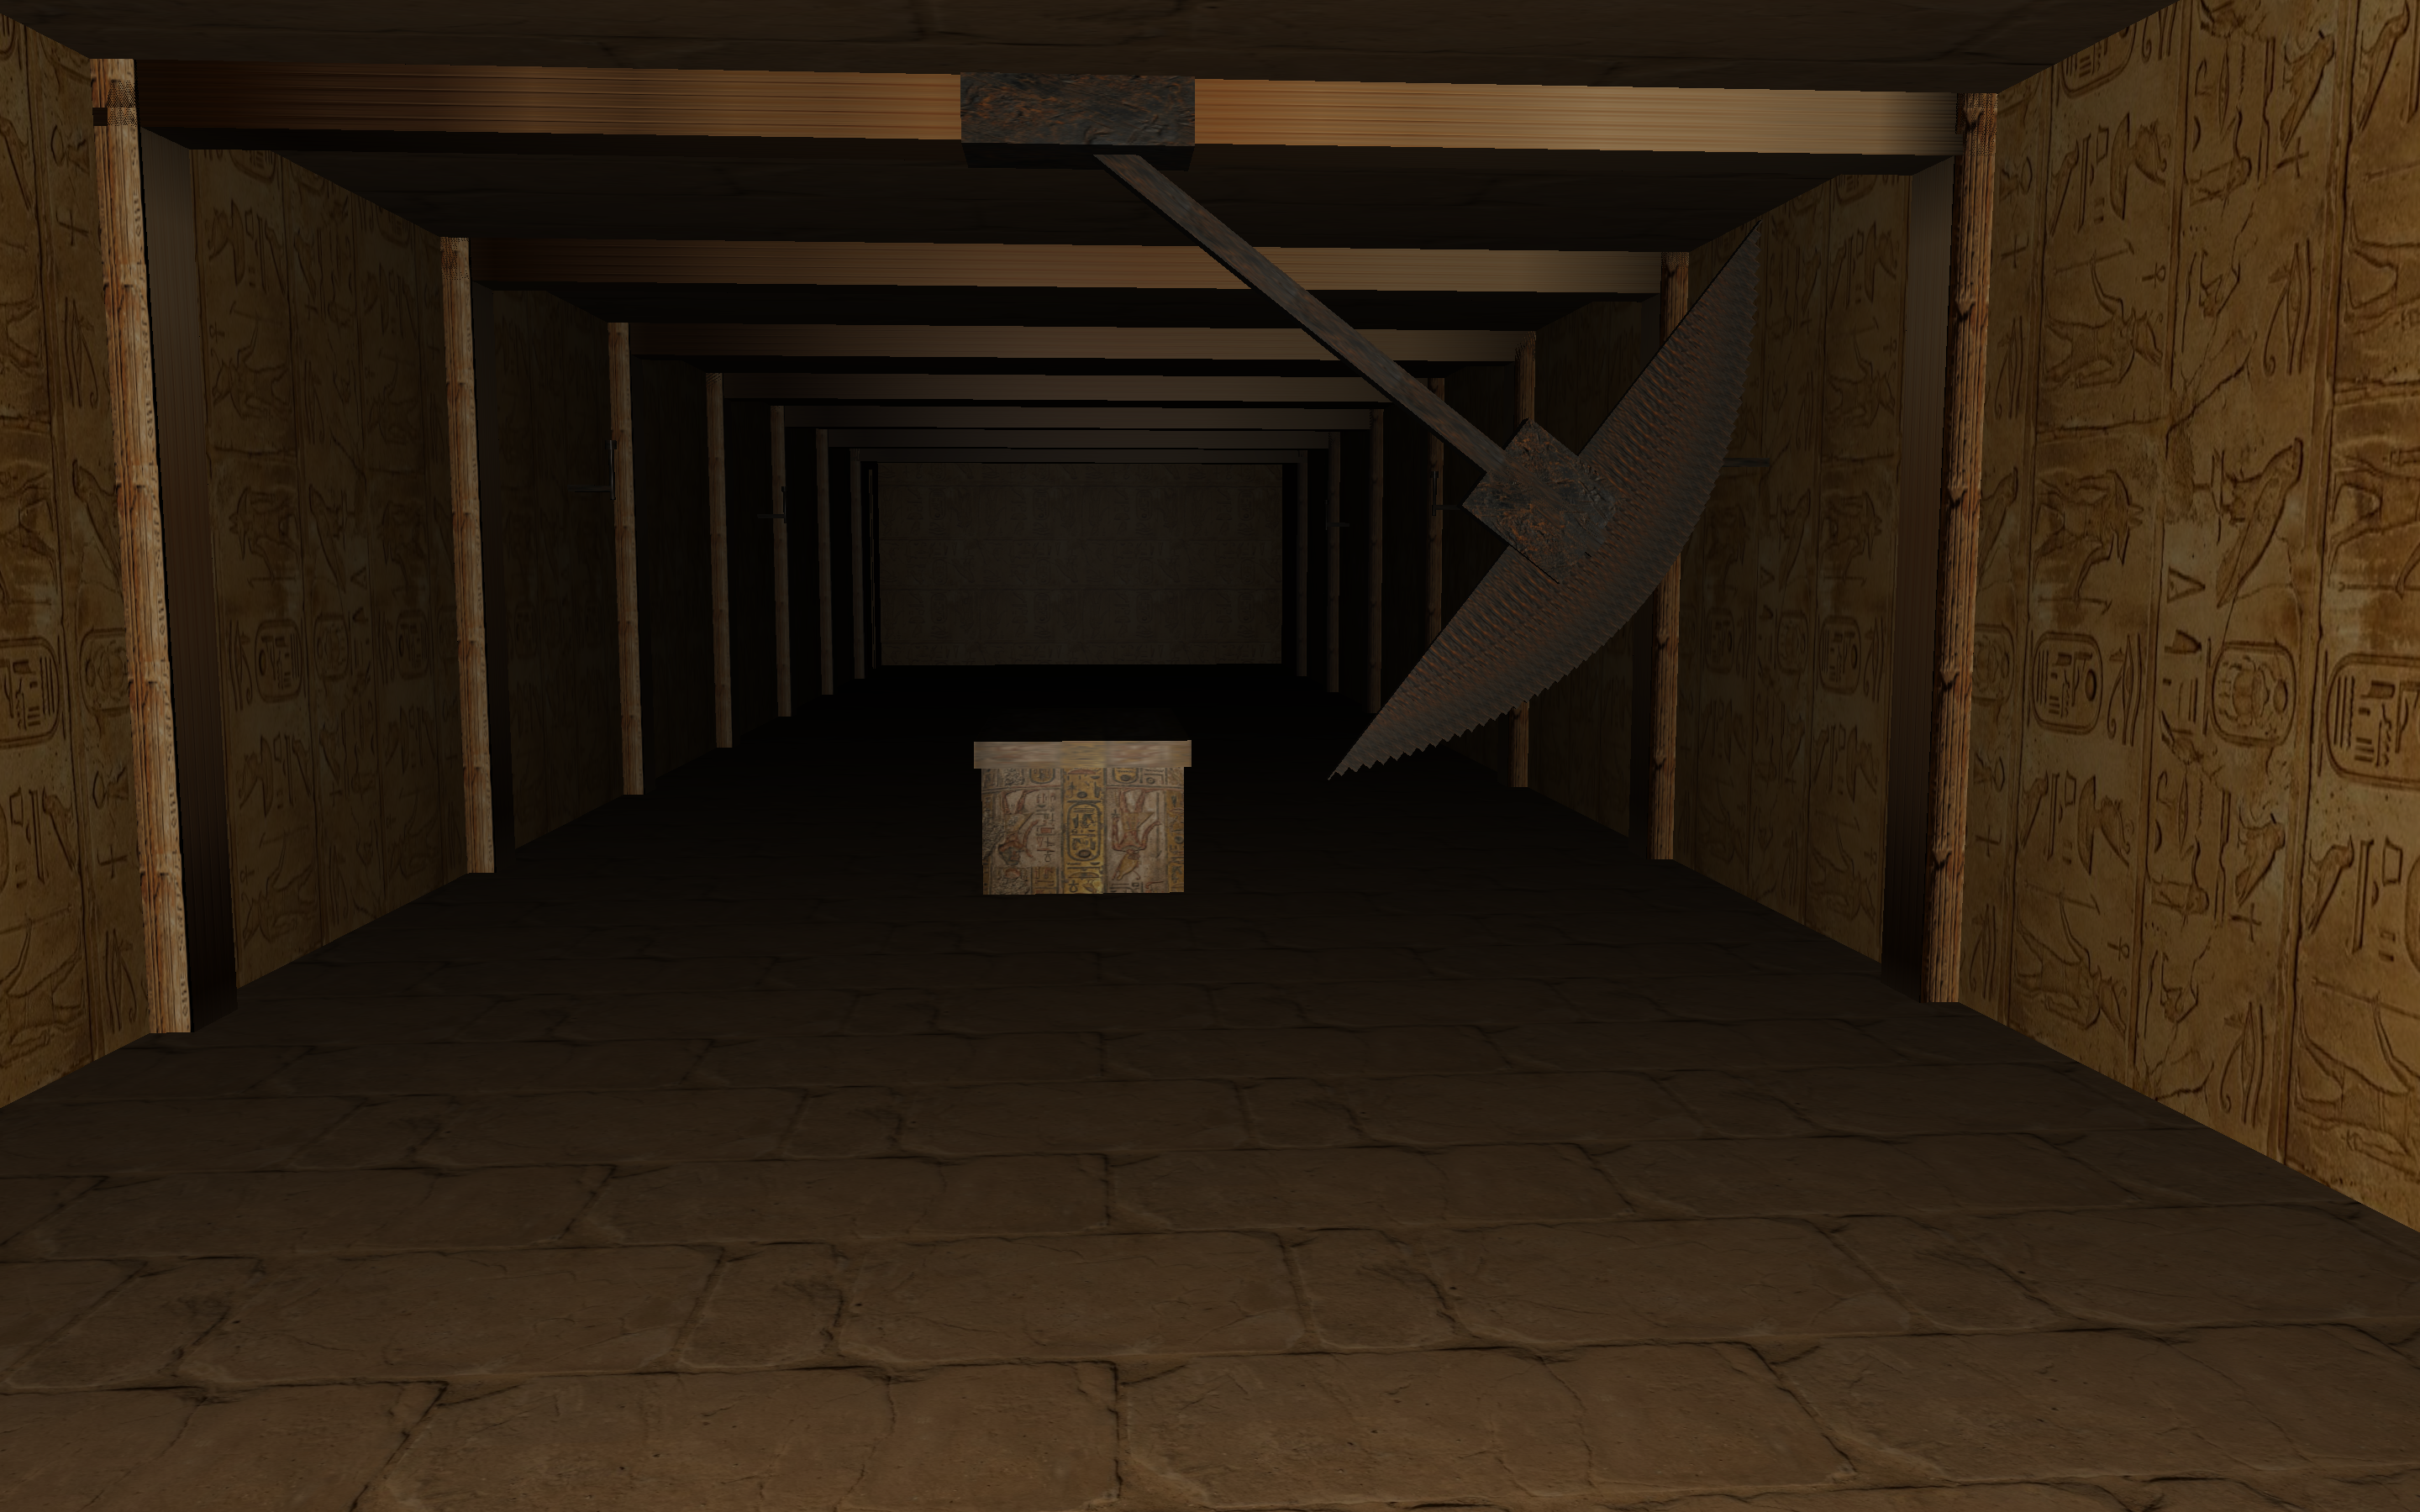
\includegraphics[width=0.9\textwidth]{screenshots/9.png}
    \caption{A demonstration of the interactive dynamic Pendulum Blade Trap descending exactly inside the user collision path, relying continuously on complex Matrix Stacking physics transferring hierarchical axis evaluations across the moving pivot frames seamlessly.}
    \label{fig:swinging_blade}
\end{figure}

\newpage

\begin{figure}[H]
    \centering
    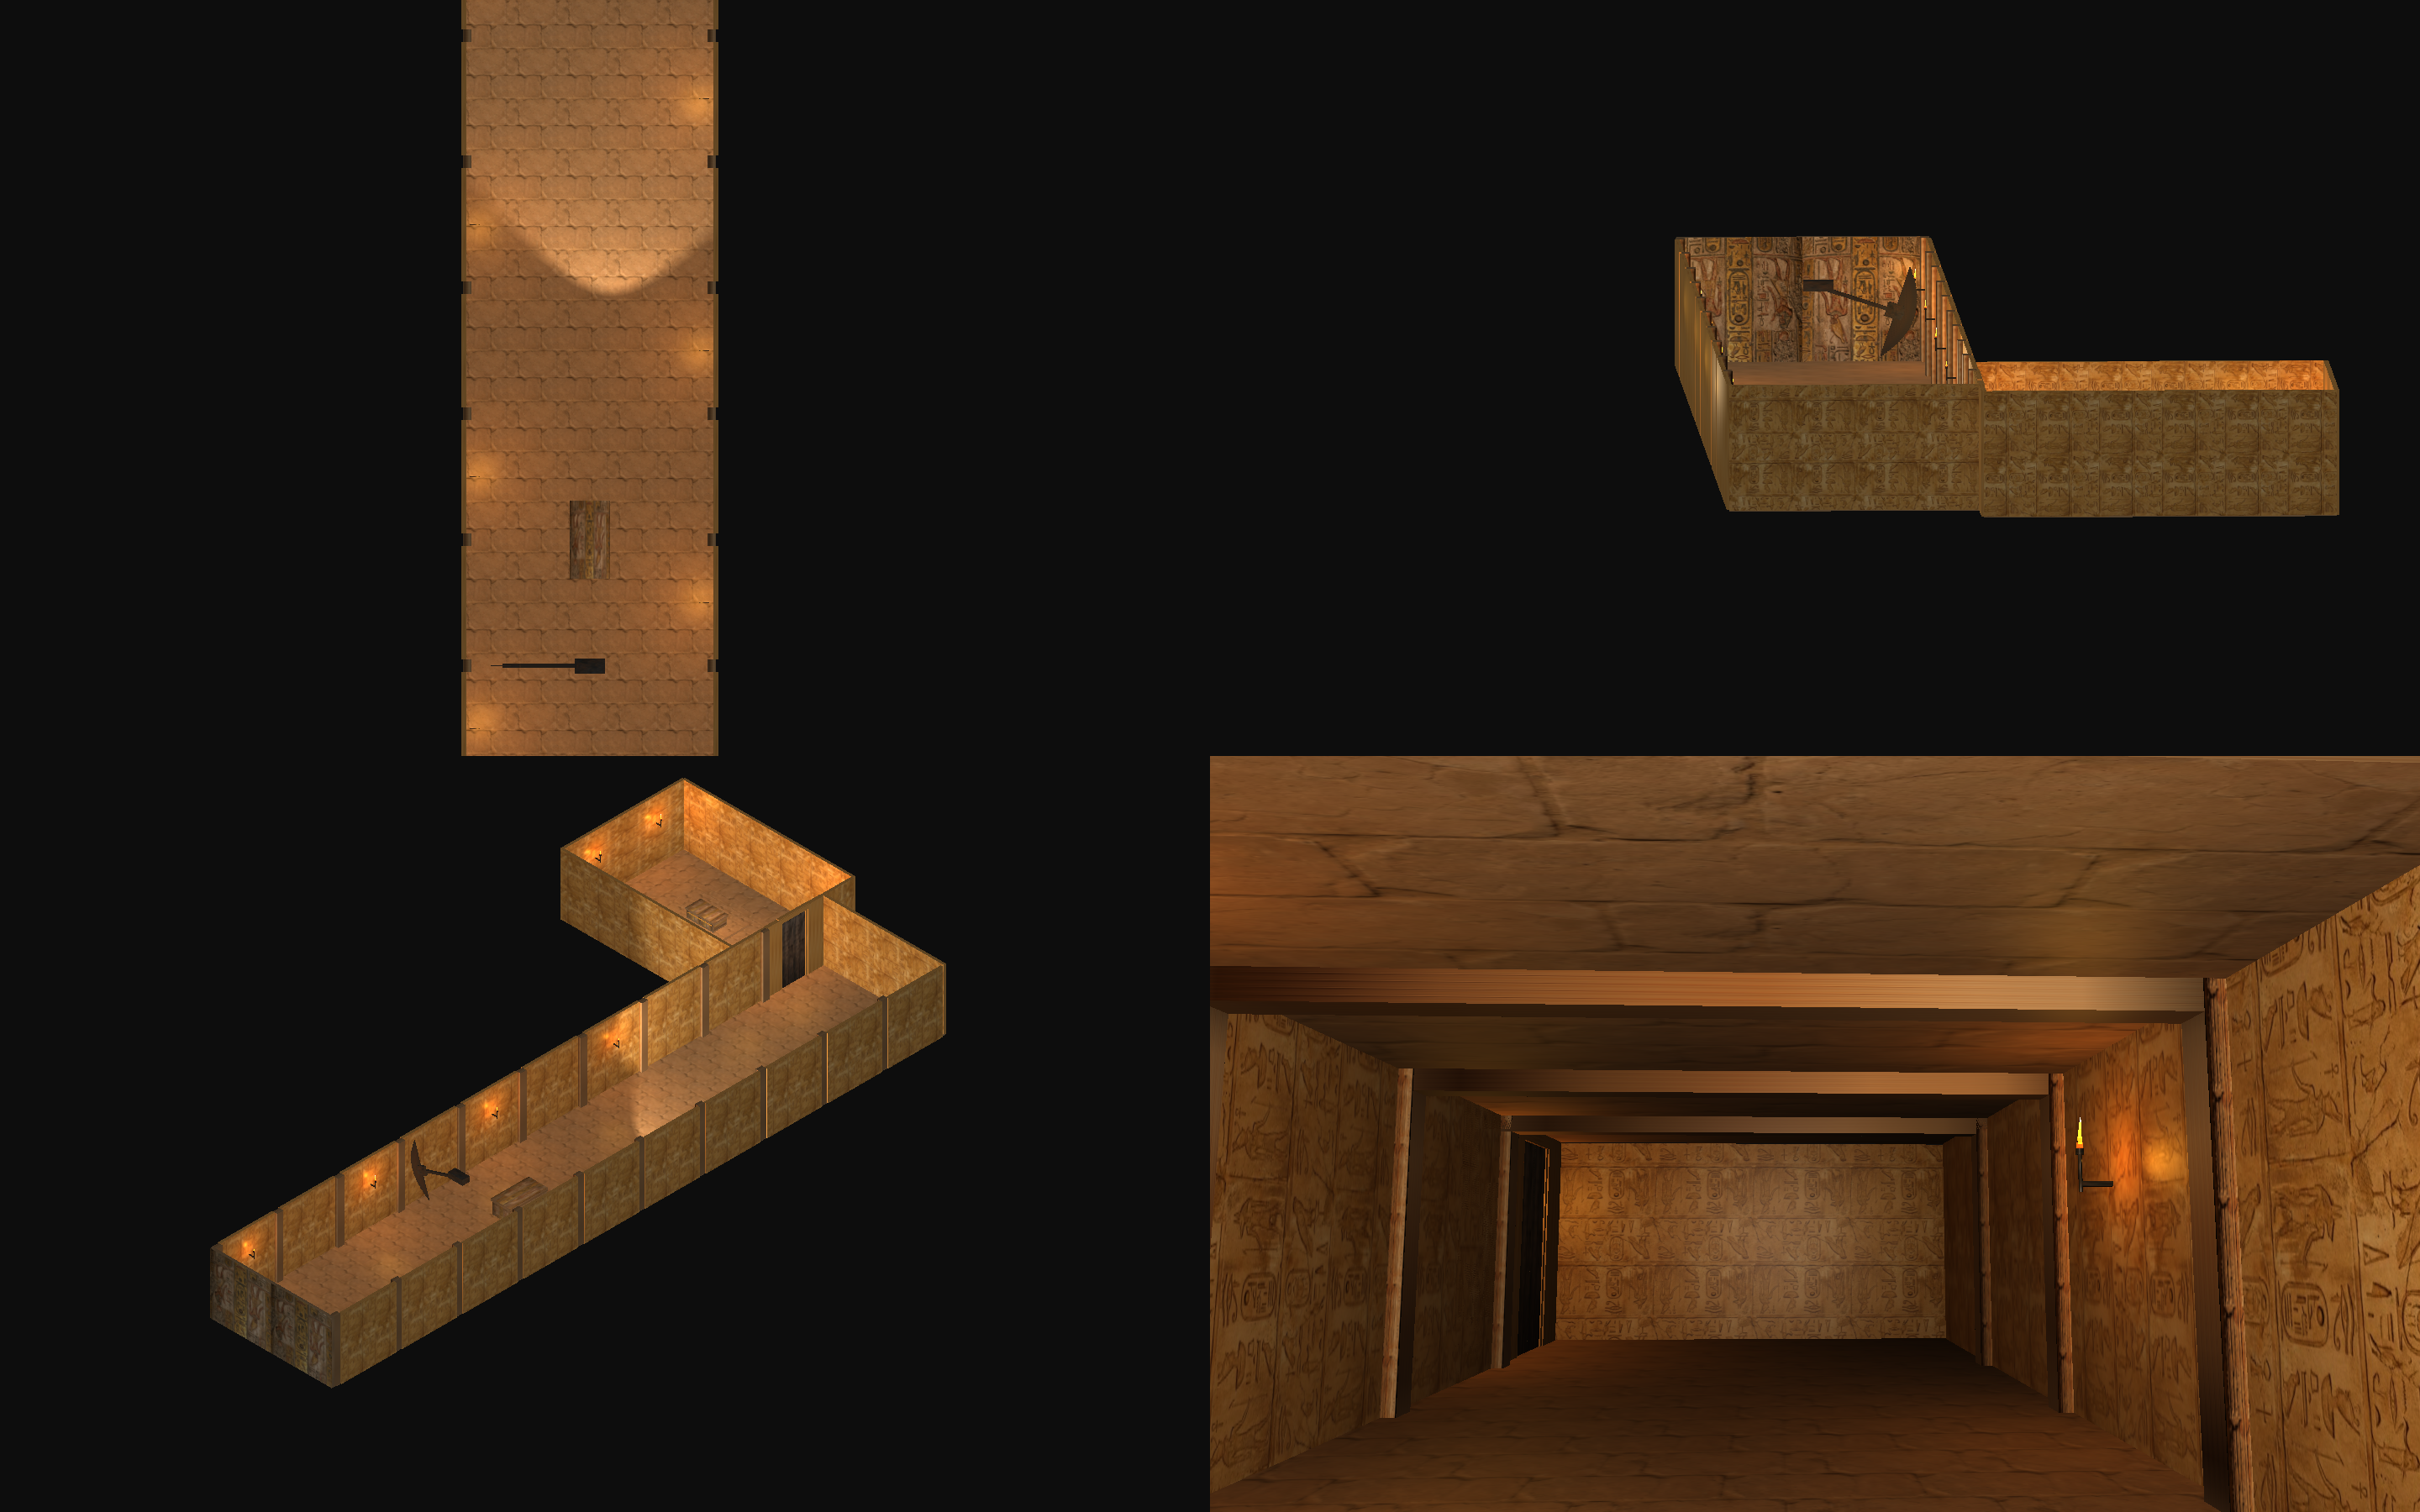
\includegraphics[width=0.9\textwidth]{screenshots/10.png}
    \caption{Dynamic multi-viewport mechanisms updating standard projections independently. Illustrating the concurrent real-time execution of Top Orthographic scaling, Isometric tracking, Perspective FPS representation, and structural side boundaries synchronously.}
    \label{fig:viewport}
\end{figure}

\begin{figure}[H]
    \centering
    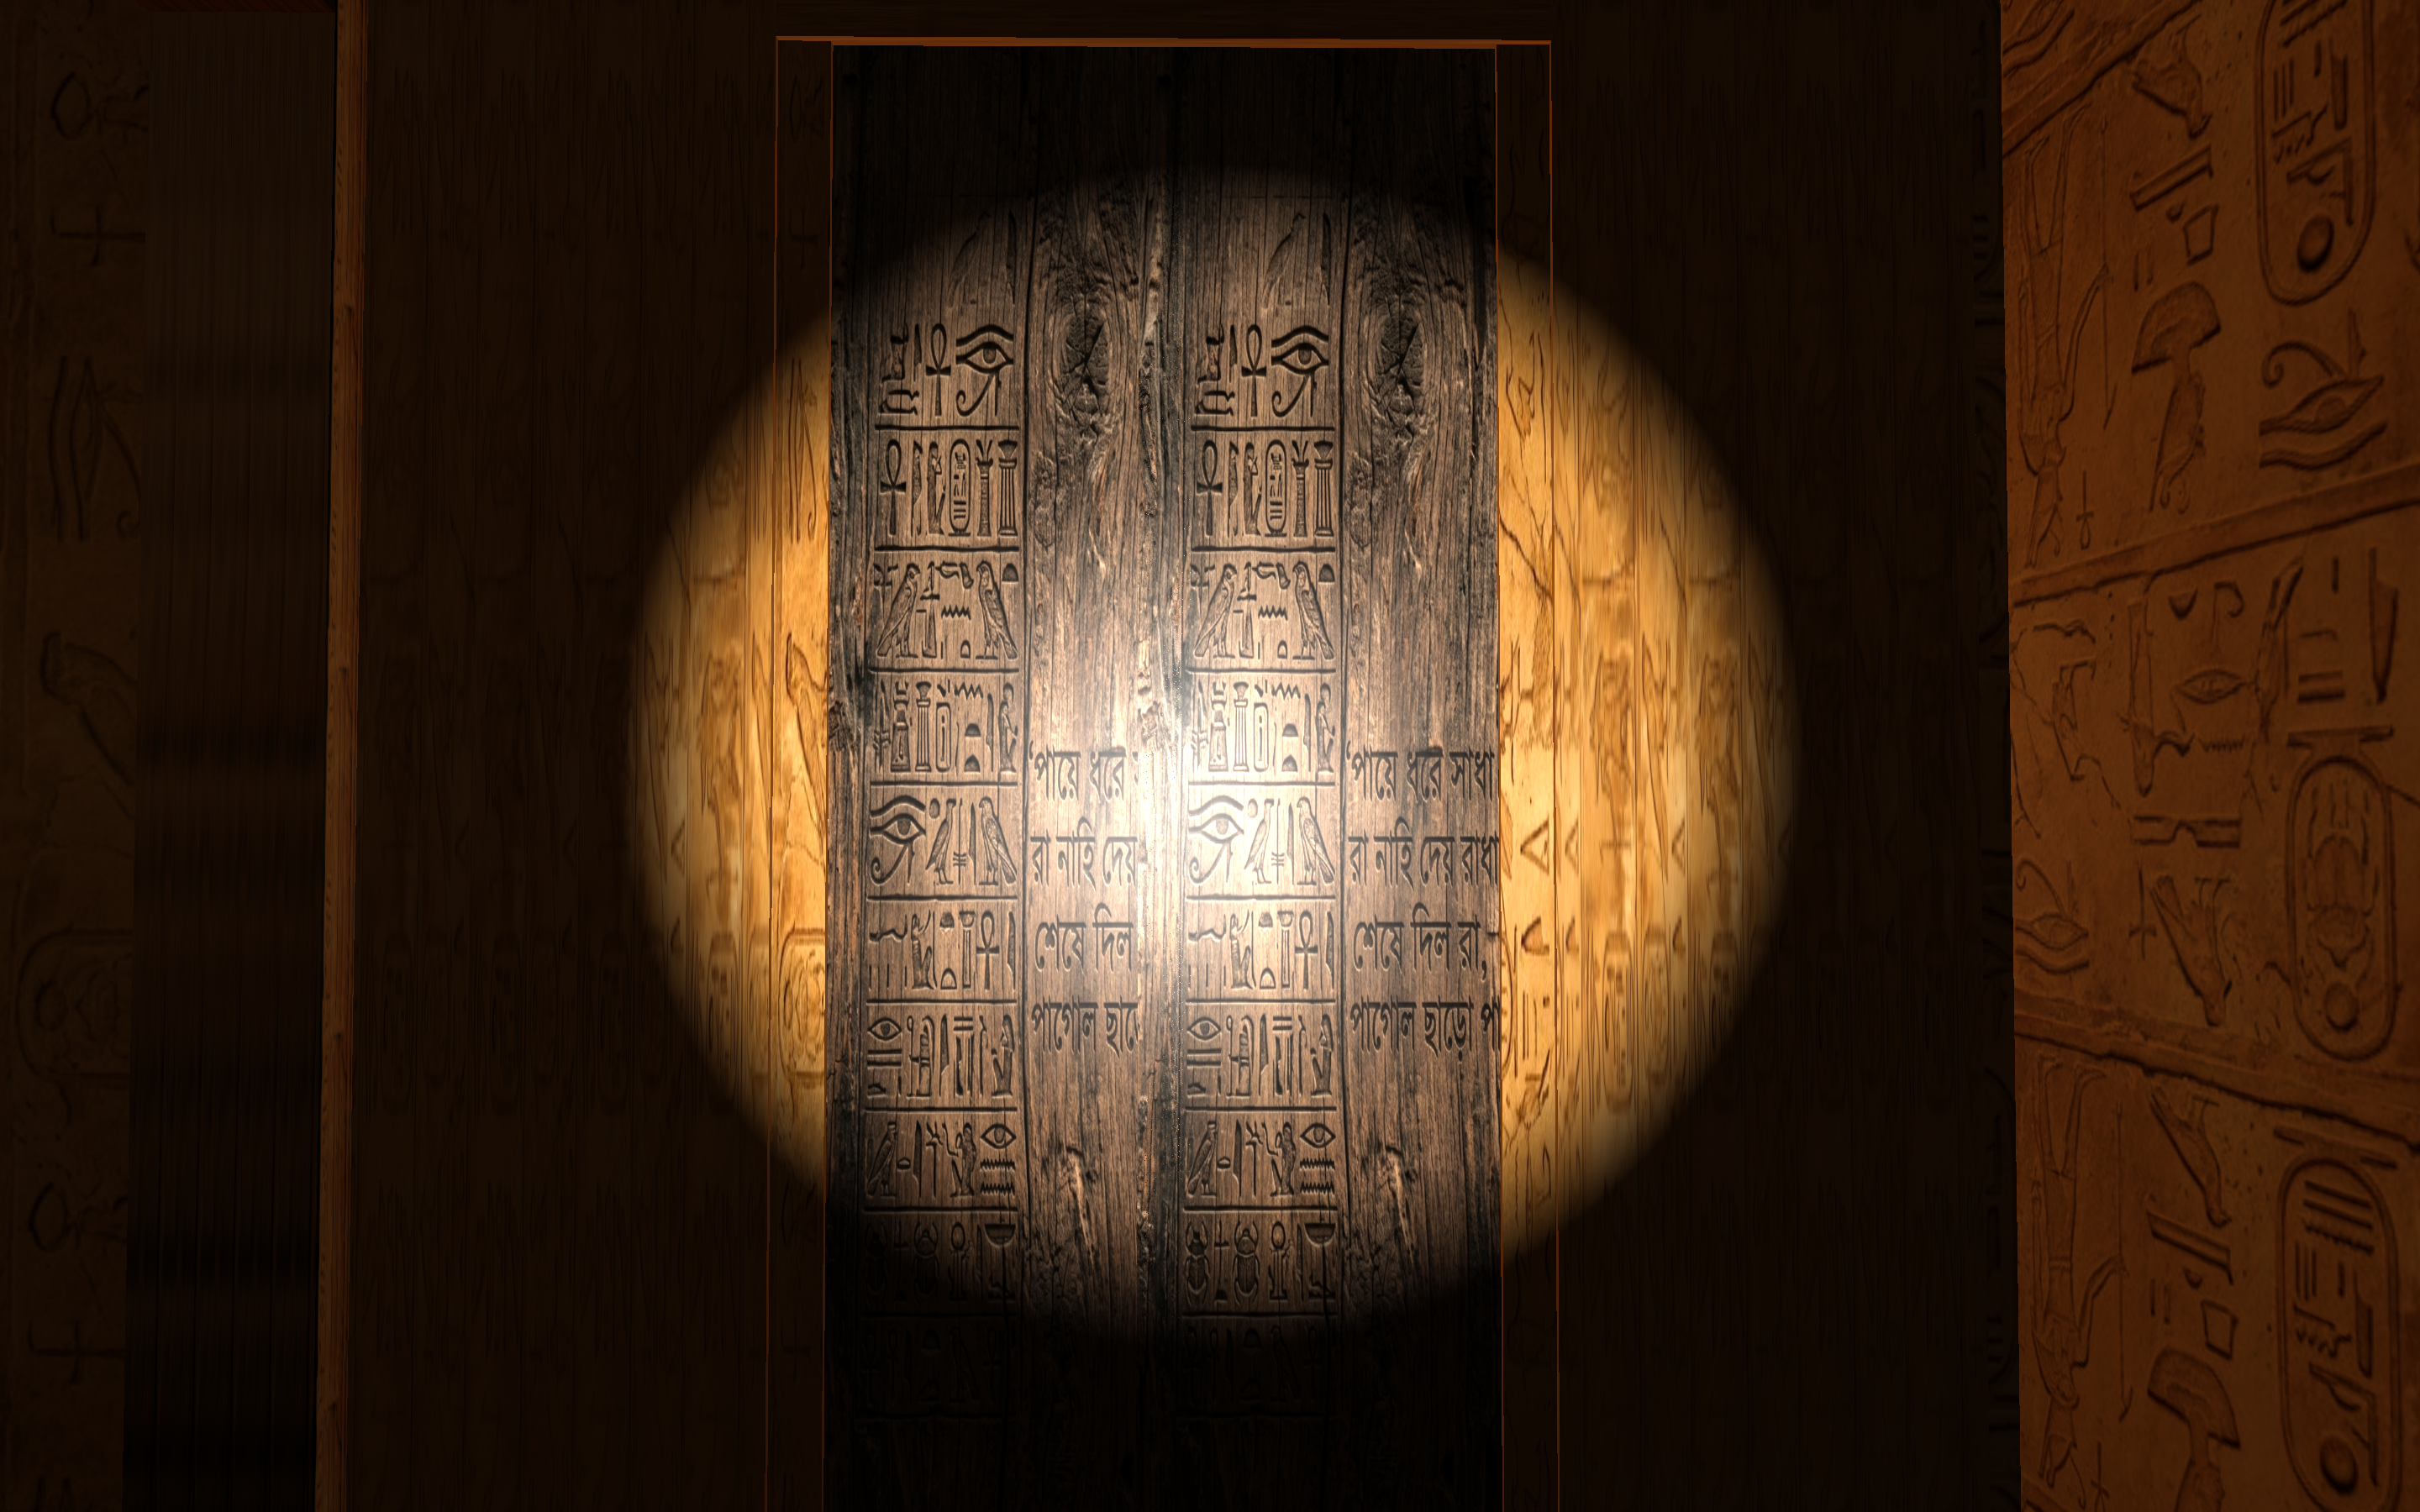
\includegraphics[width=0.9\textwidth]{screenshots/11.png}
    \caption{The Spotlight mechanism (Flashlight) focusing a precisely constrained illuminating cone angle over a complex hieroglyphic textured wall frame, demonstrating exact dot-product clipping bounds calculated inside the active fragment shader strictly resolving pixel visibility natively.}
    \label{fig:hieroglyph_spotlight}
\end{figure}

\newpage

\begin{figure}[H]
    \centering
    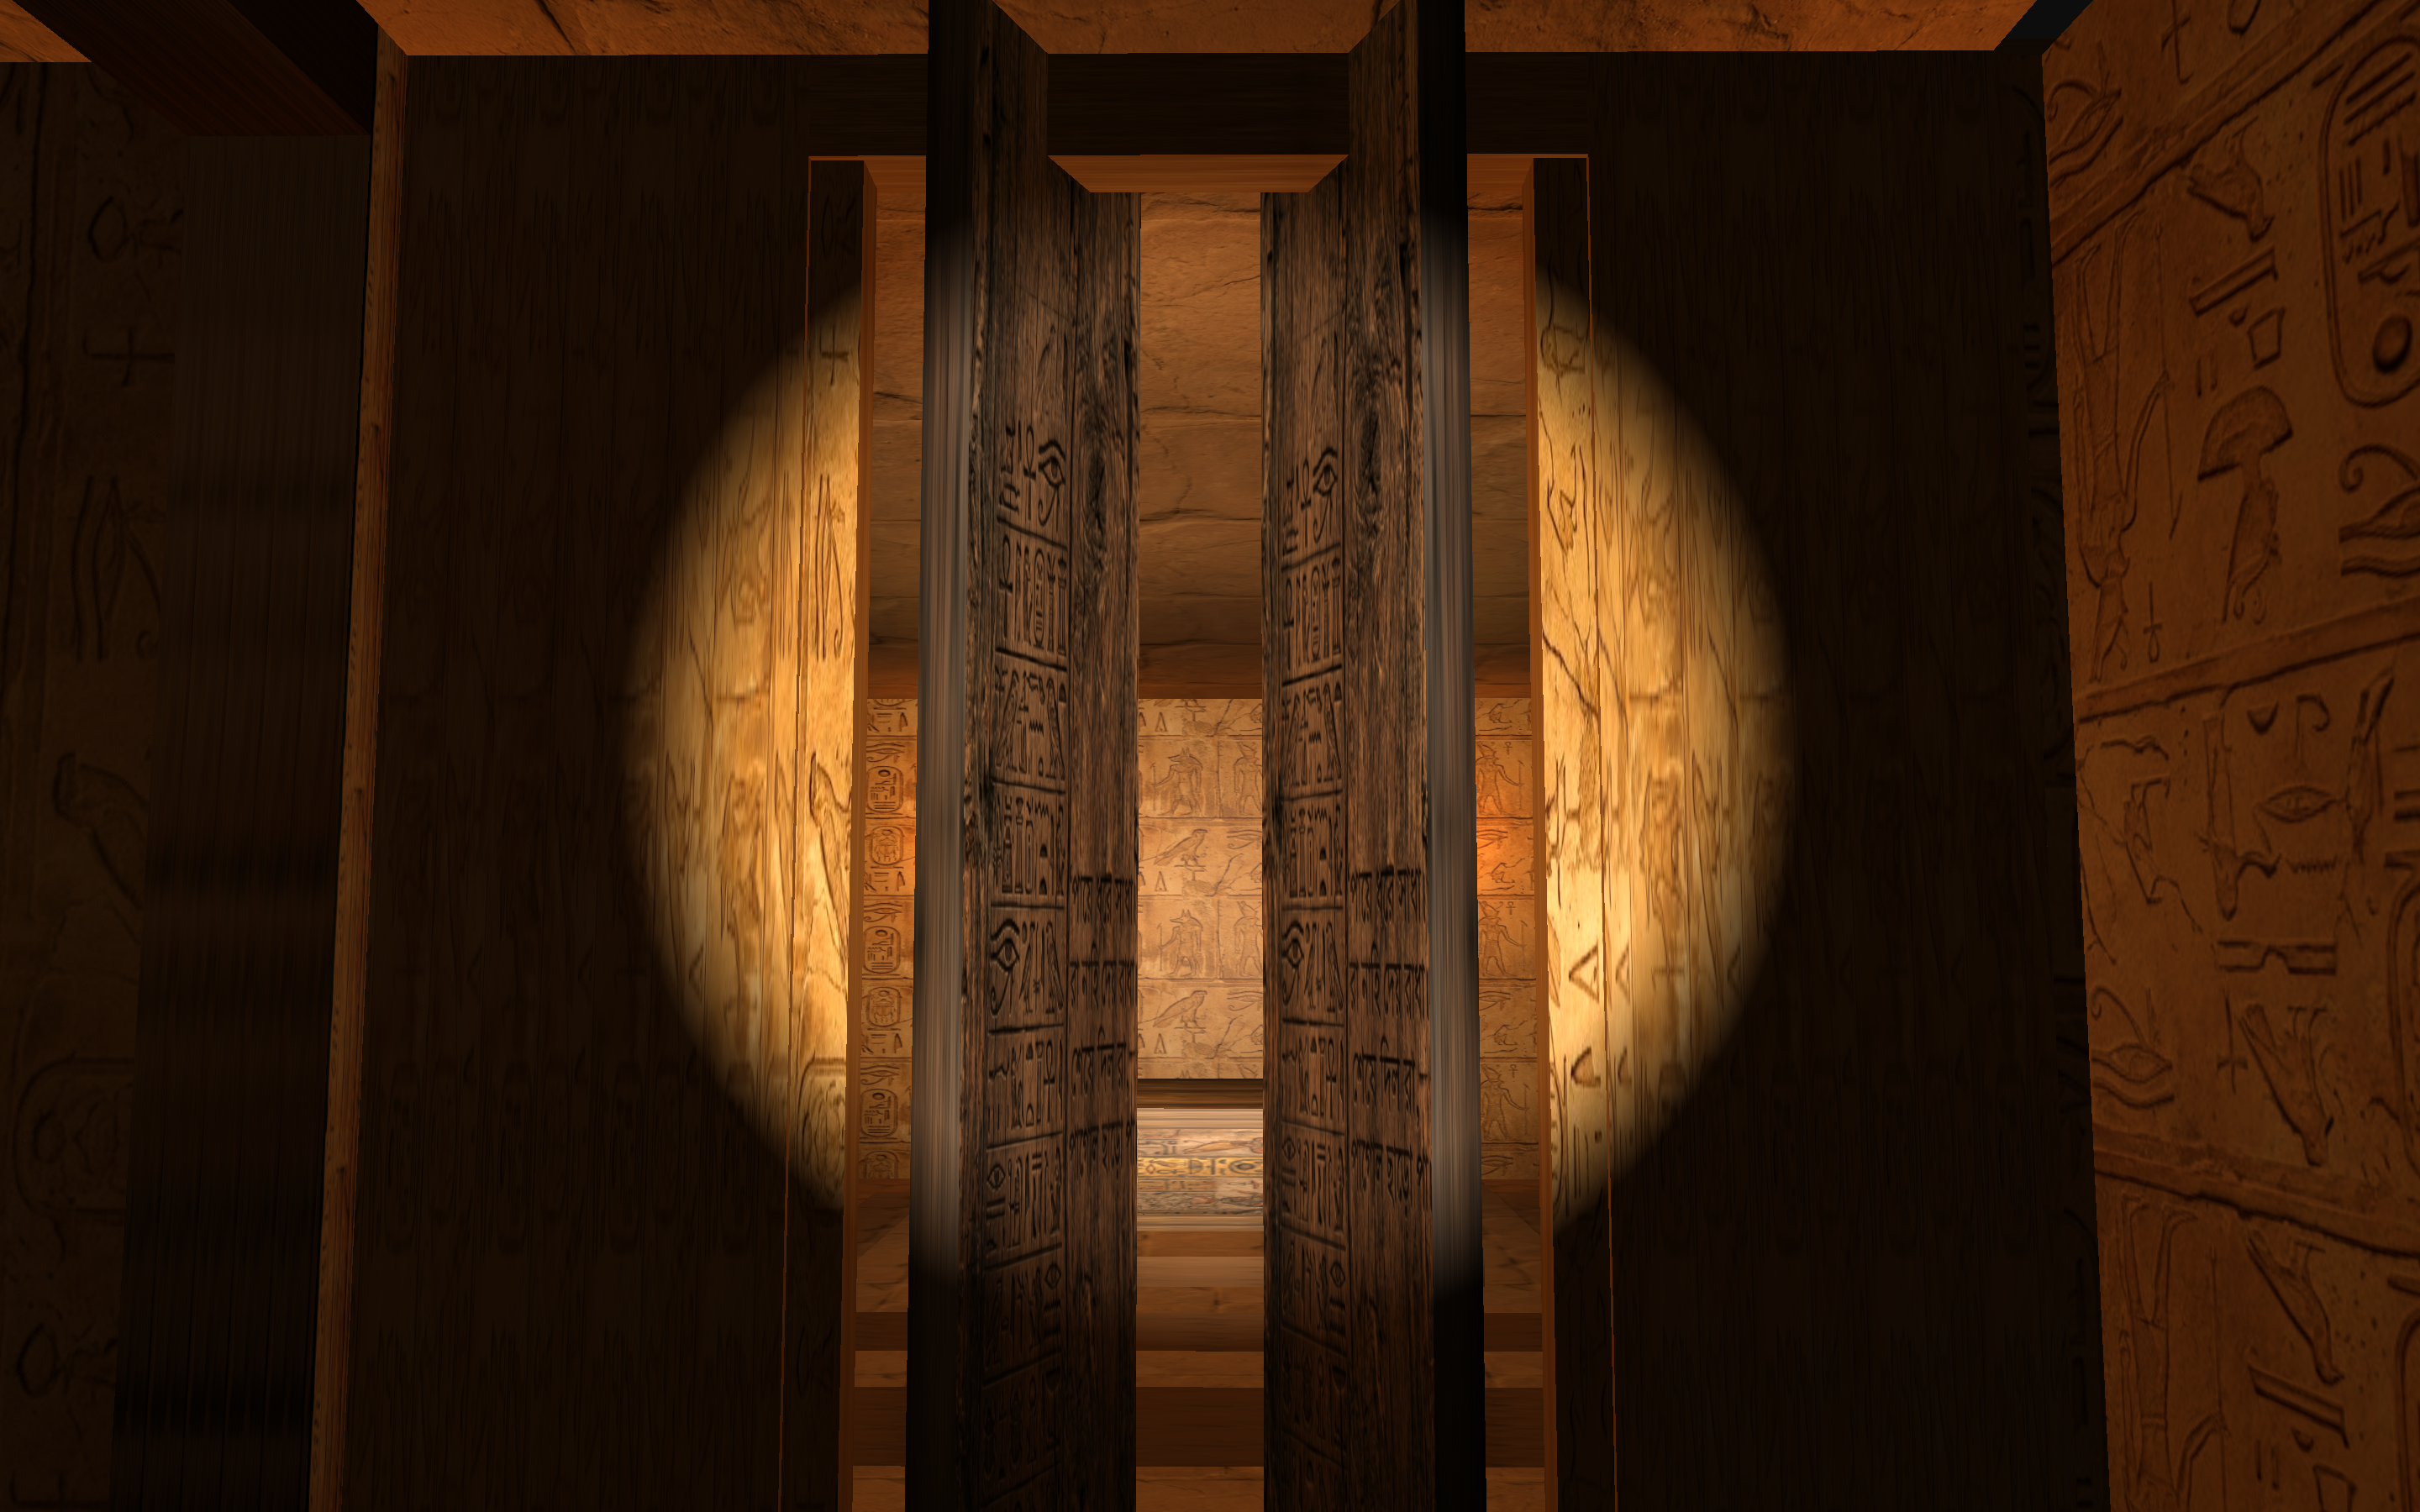
\includegraphics[width=0.9\textwidth]{screenshots/12.png}
    \caption{The primary structural passage doors lit selectively via tight spotlight configurations, casting highly defined directional boundaries whilst preserving immersive peripheral ambient shadow mapping entirely rendering the dark architectural bounds effectively.}
    \label{fig:passage_door}
\end{figure}

\begin{figure}[H]
    \centering
    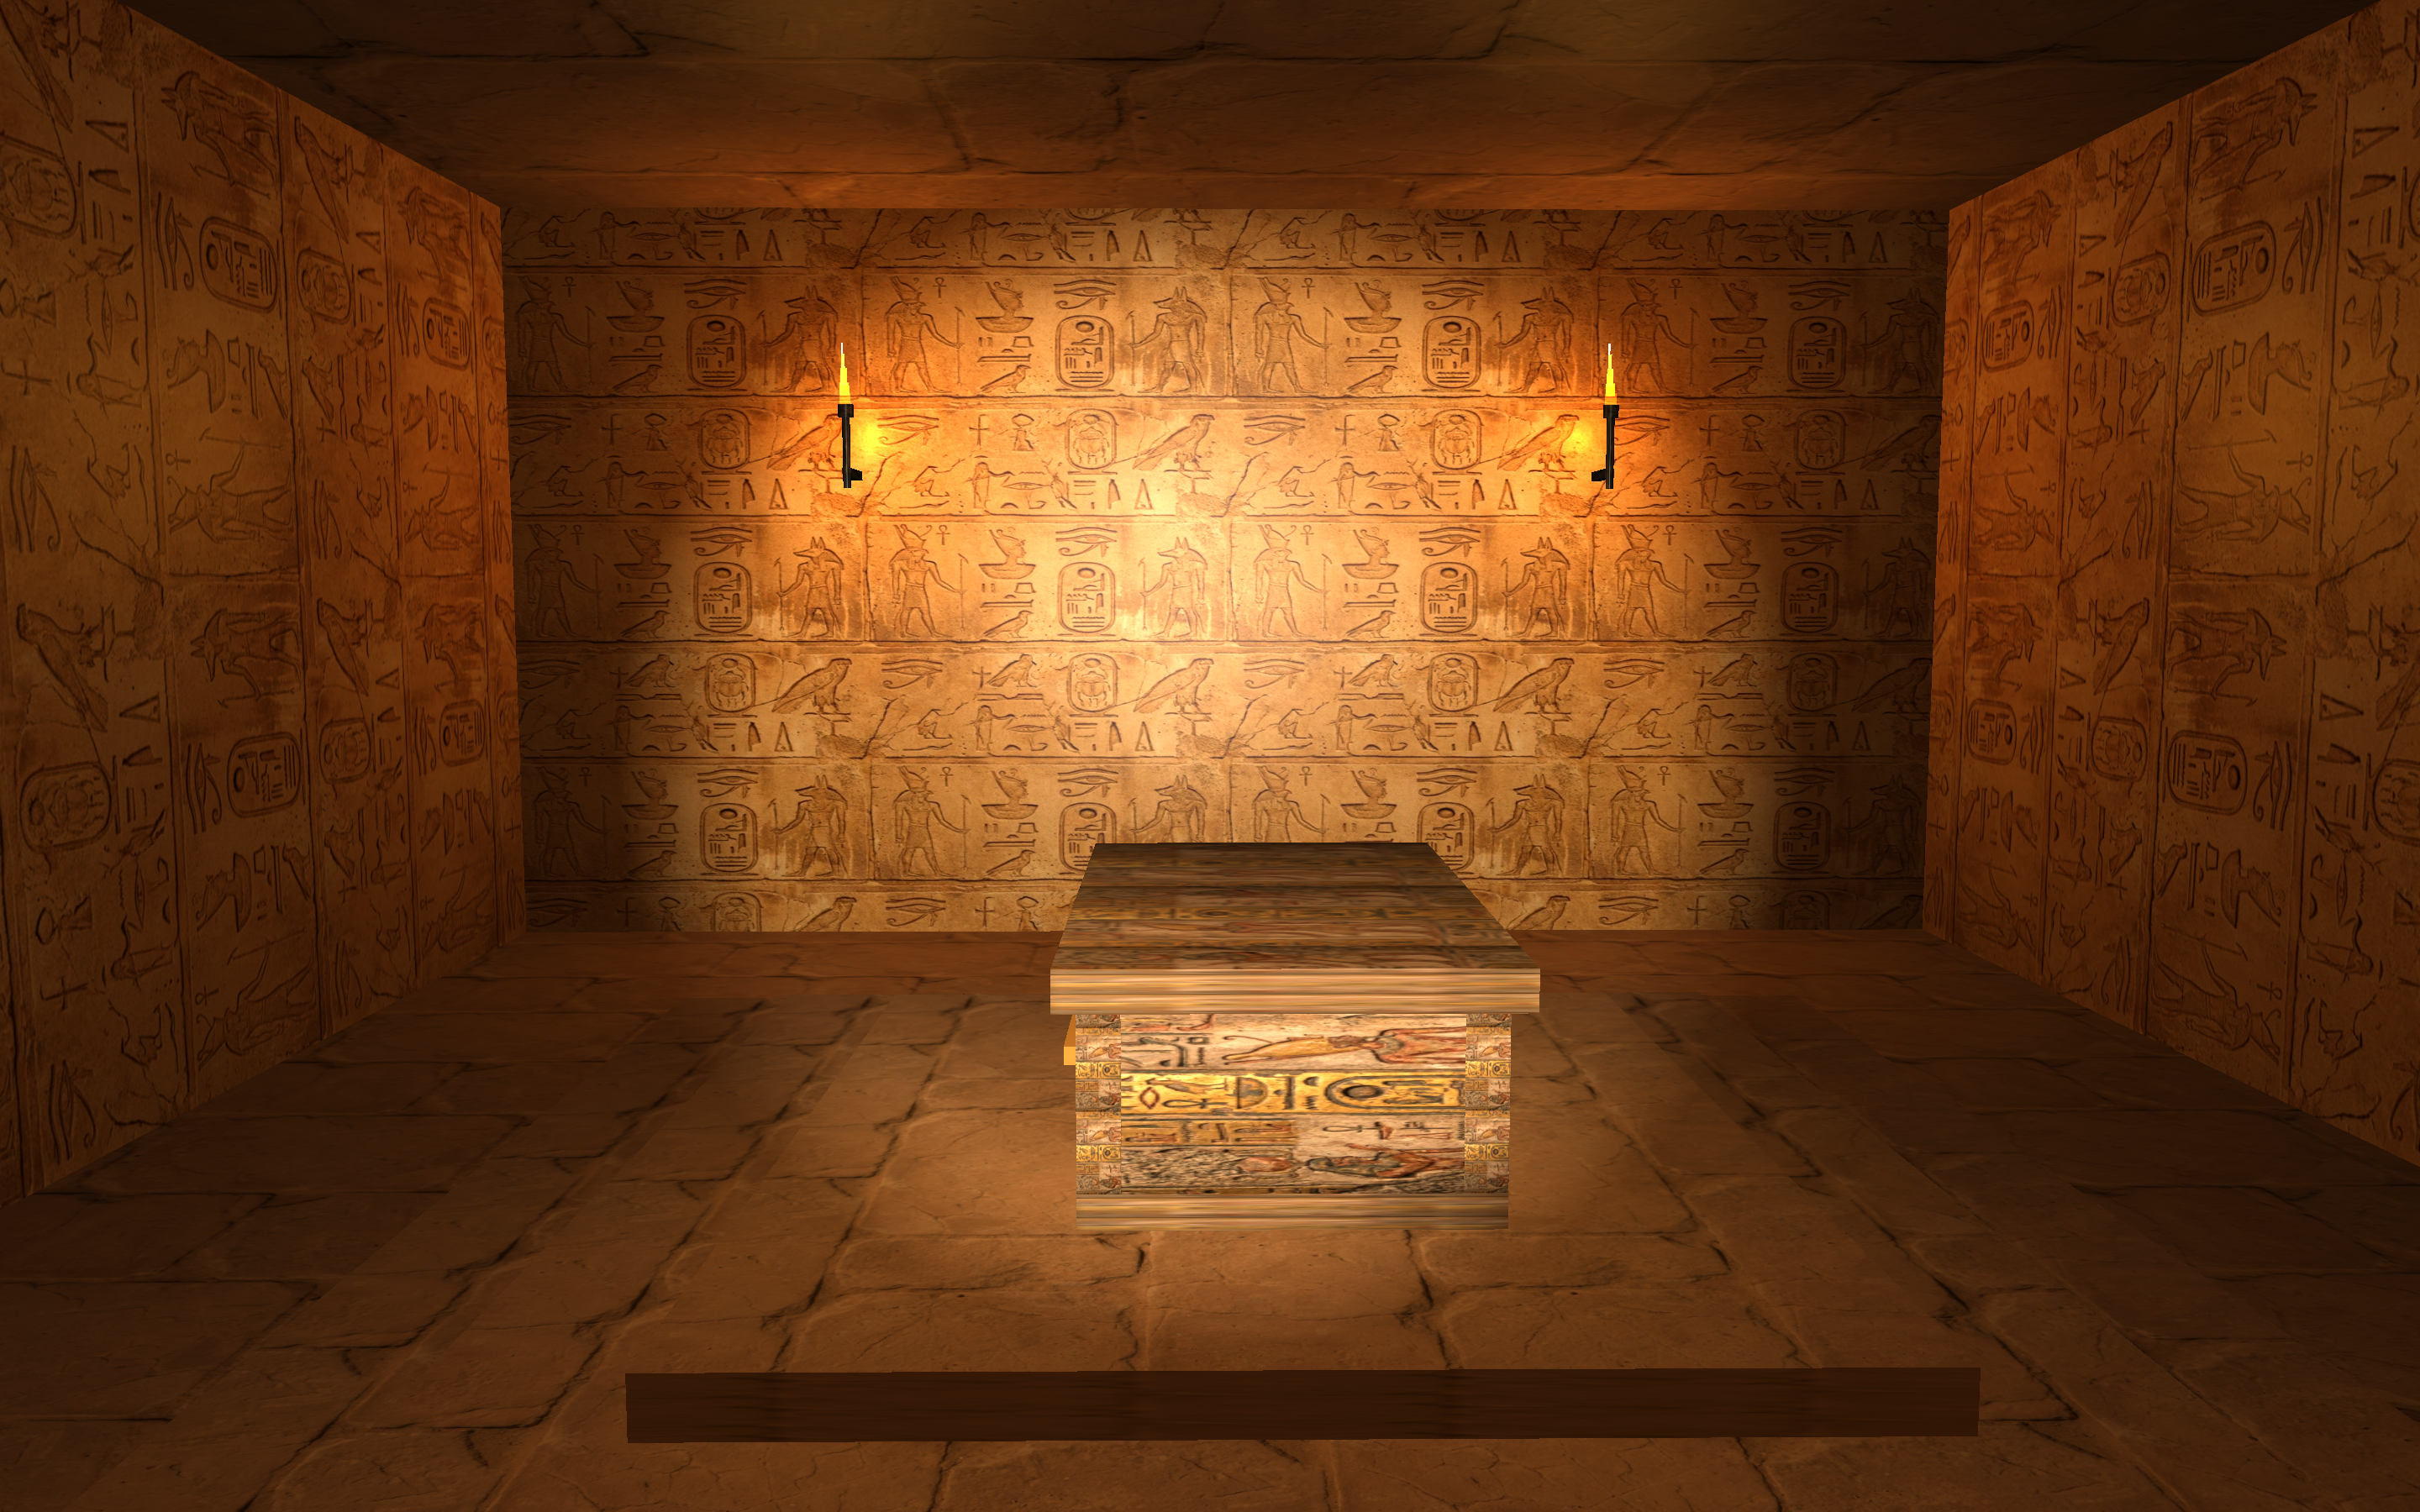
\includegraphics[width=0.9\textwidth]{screenshots/13.png}
    \caption{The Grand Burial Chamber displaying standard multi-light overlaps. Symmetrical Lantern Point-lights gracefully scatter mapped specular reflections cascading across textual overlays mapping the historical hieroglyph wall elements surrounding the static sarcophagus.}
    \label{fig:burial_chamber}
\end{figure}

\newpage

\begin{figure}[H]
    \centering
    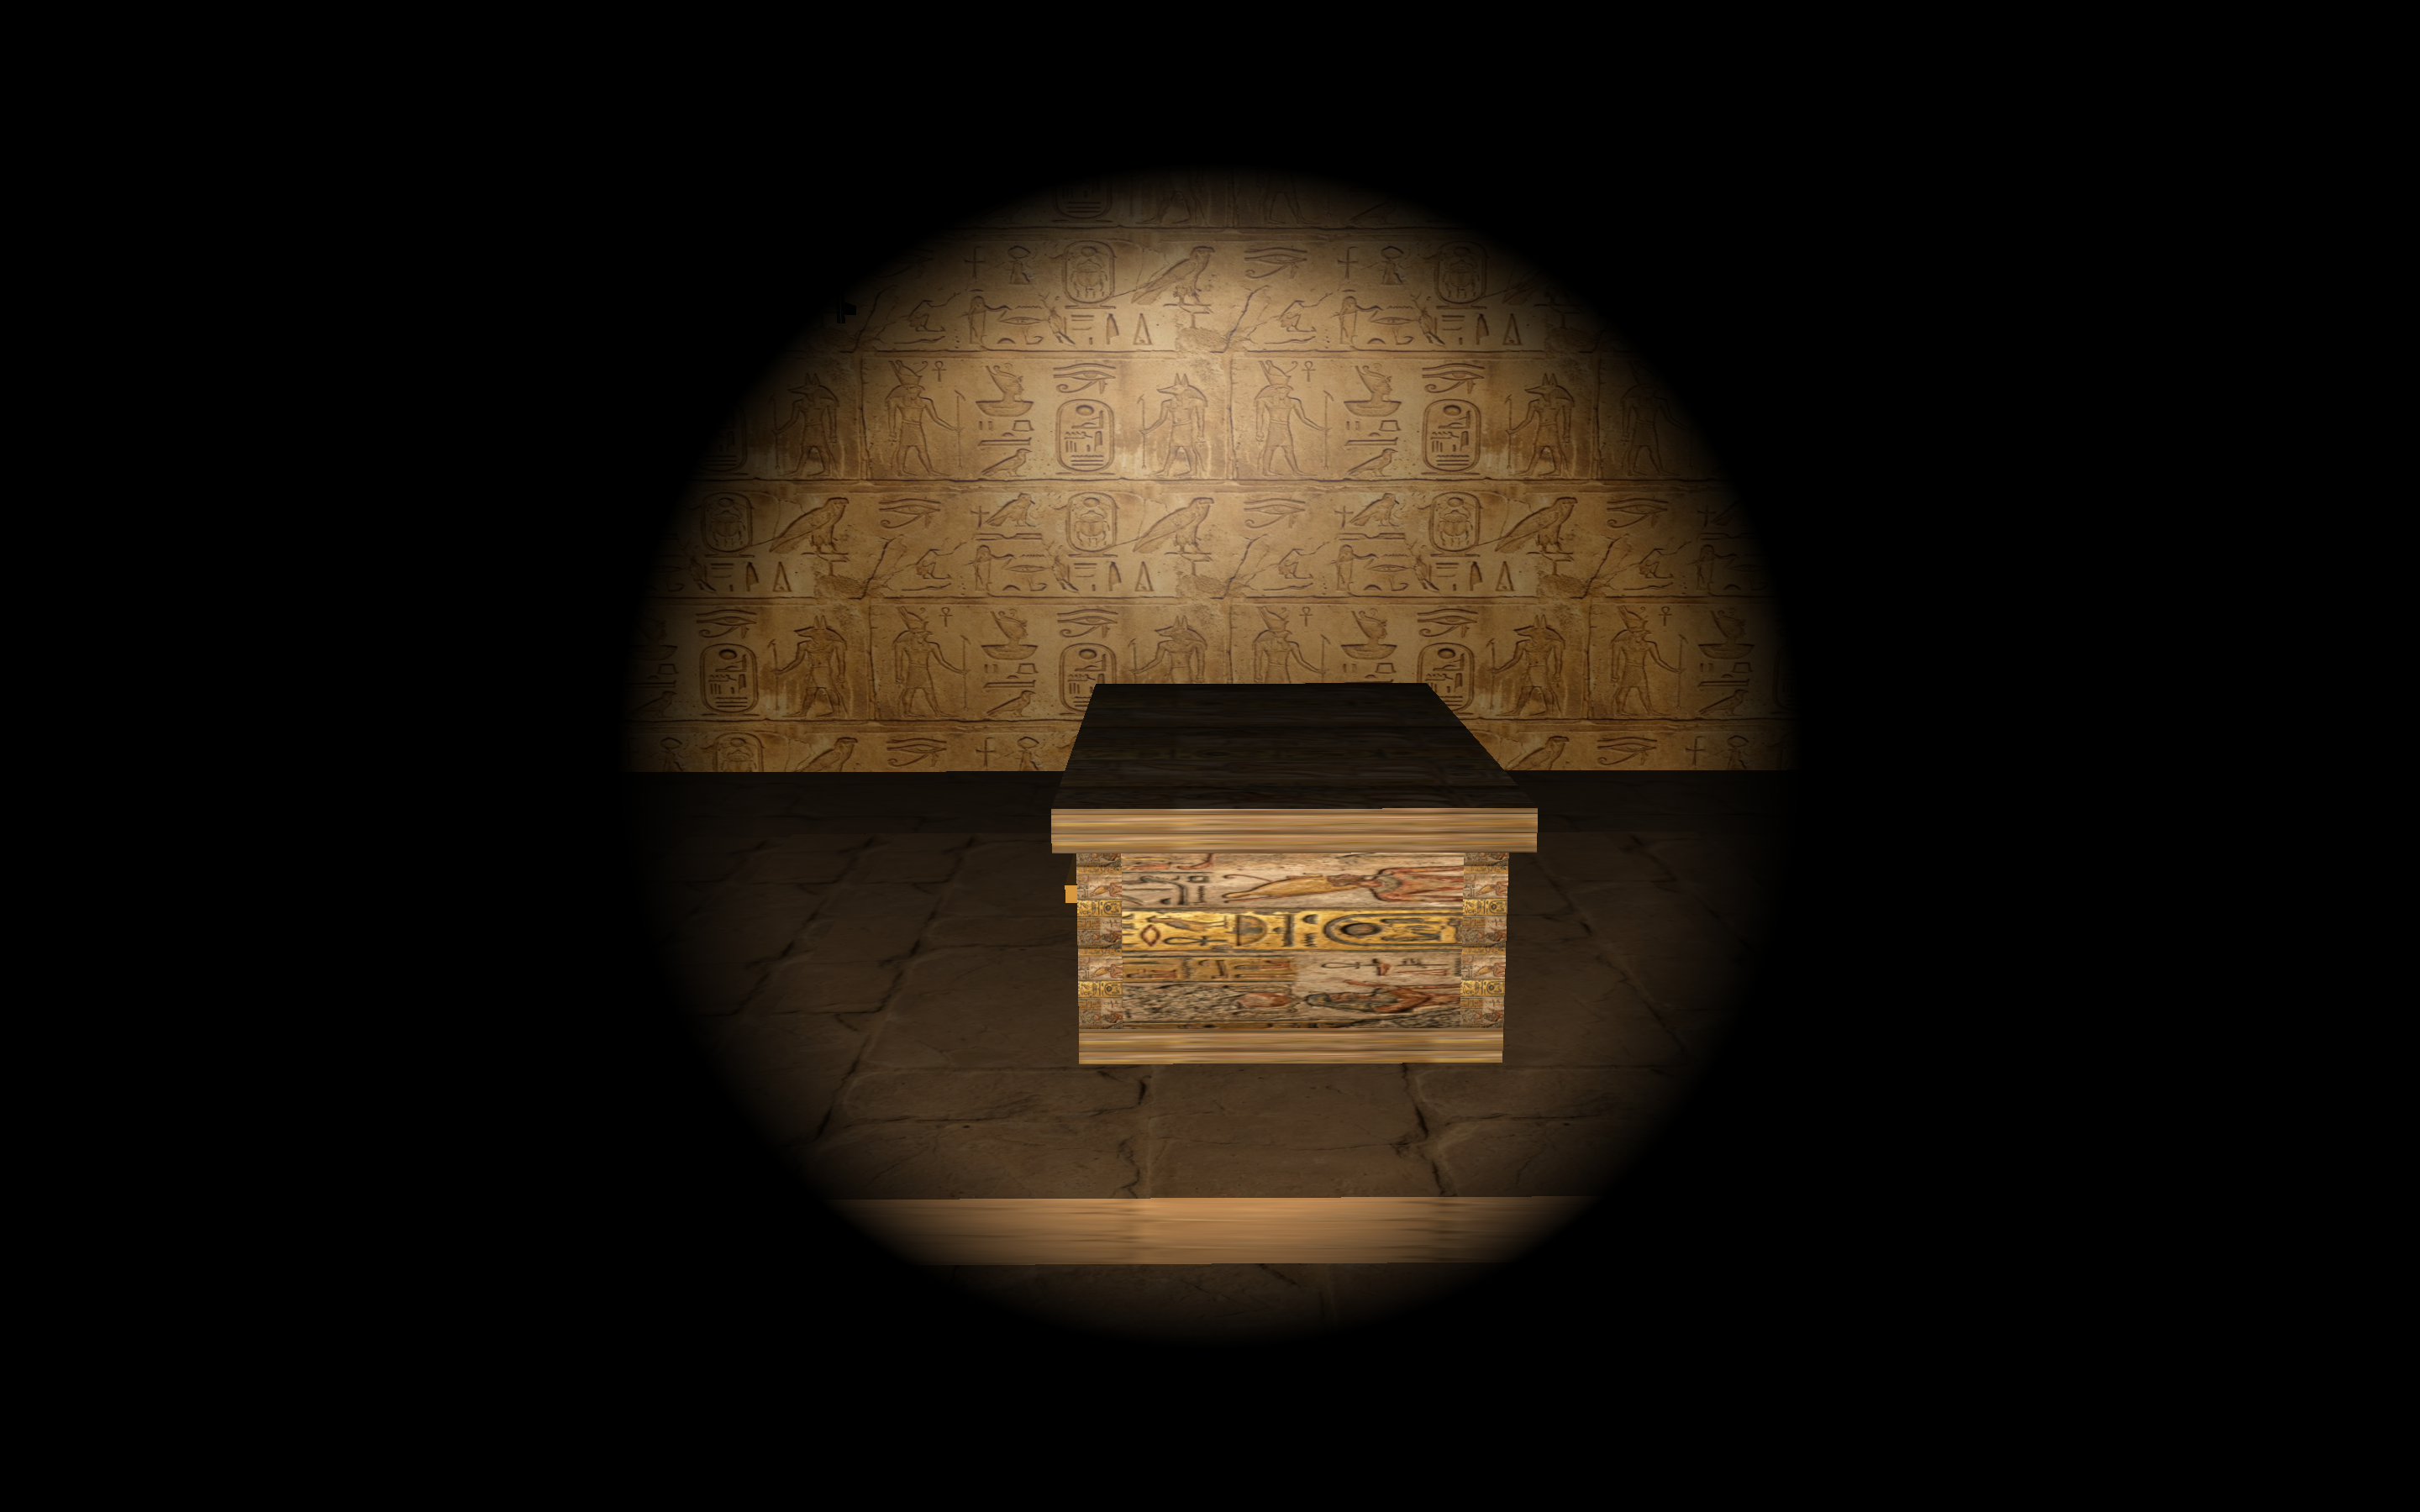
\includegraphics[width=0.9\textwidth]{screenshots/14.png}
    \caption{Selective Spot Lighting exclusively isolating the central interactive Sarcophagus mesh visually. Notice the defined strict spotlight rim cutoff scaling sharply against adjacent walls devoid of corresponding ambient bleed algorithms highlighting user tracking.}
    \label{fig:spotlight_sarcophagus}
\end{figure}

\begin{figure}[H]
    \centering
    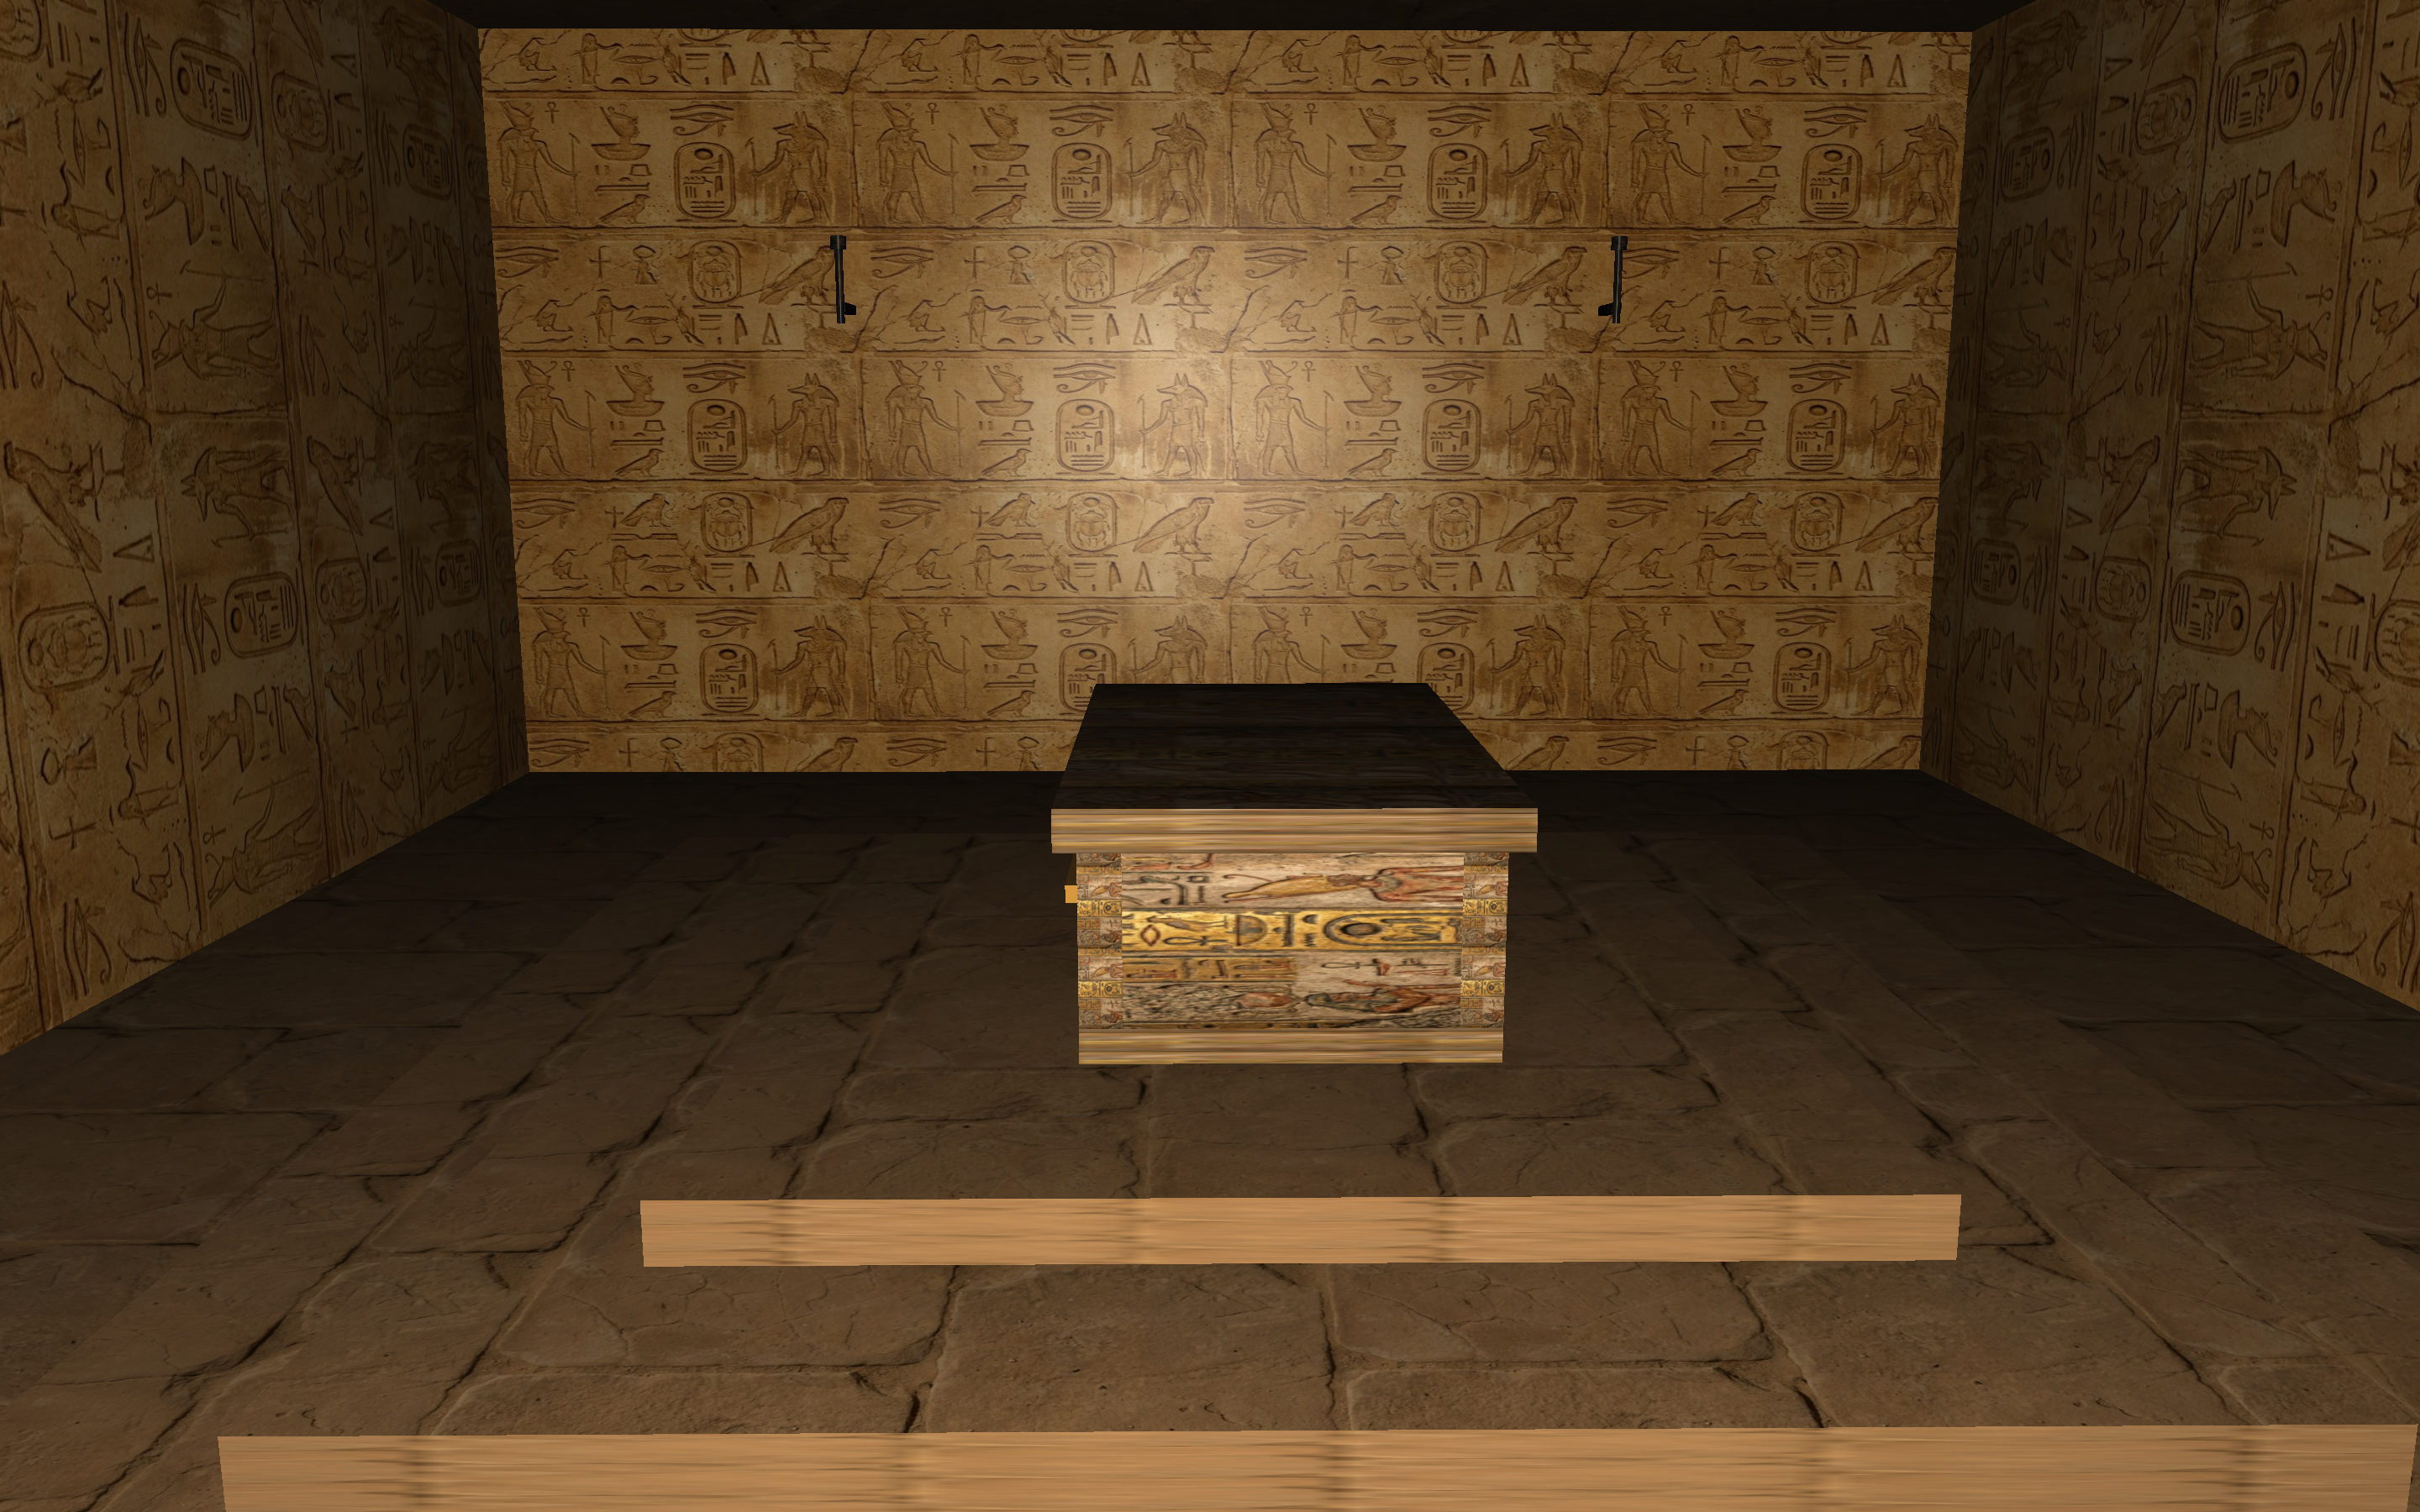
\includegraphics[width=0.9\textwidth]{screenshots/15.png}
    \caption{The unmodified Sarcophagus asset under standard constant lighting parameters to appreciate intricate bounding box construction mapping separate textual coordinates evenly prior to complex normal shading interference processes scaling.}
    \label{fig:even_sarcophagus}
\end{figure}

\newpage

\begin{figure}[H]
    \centering
    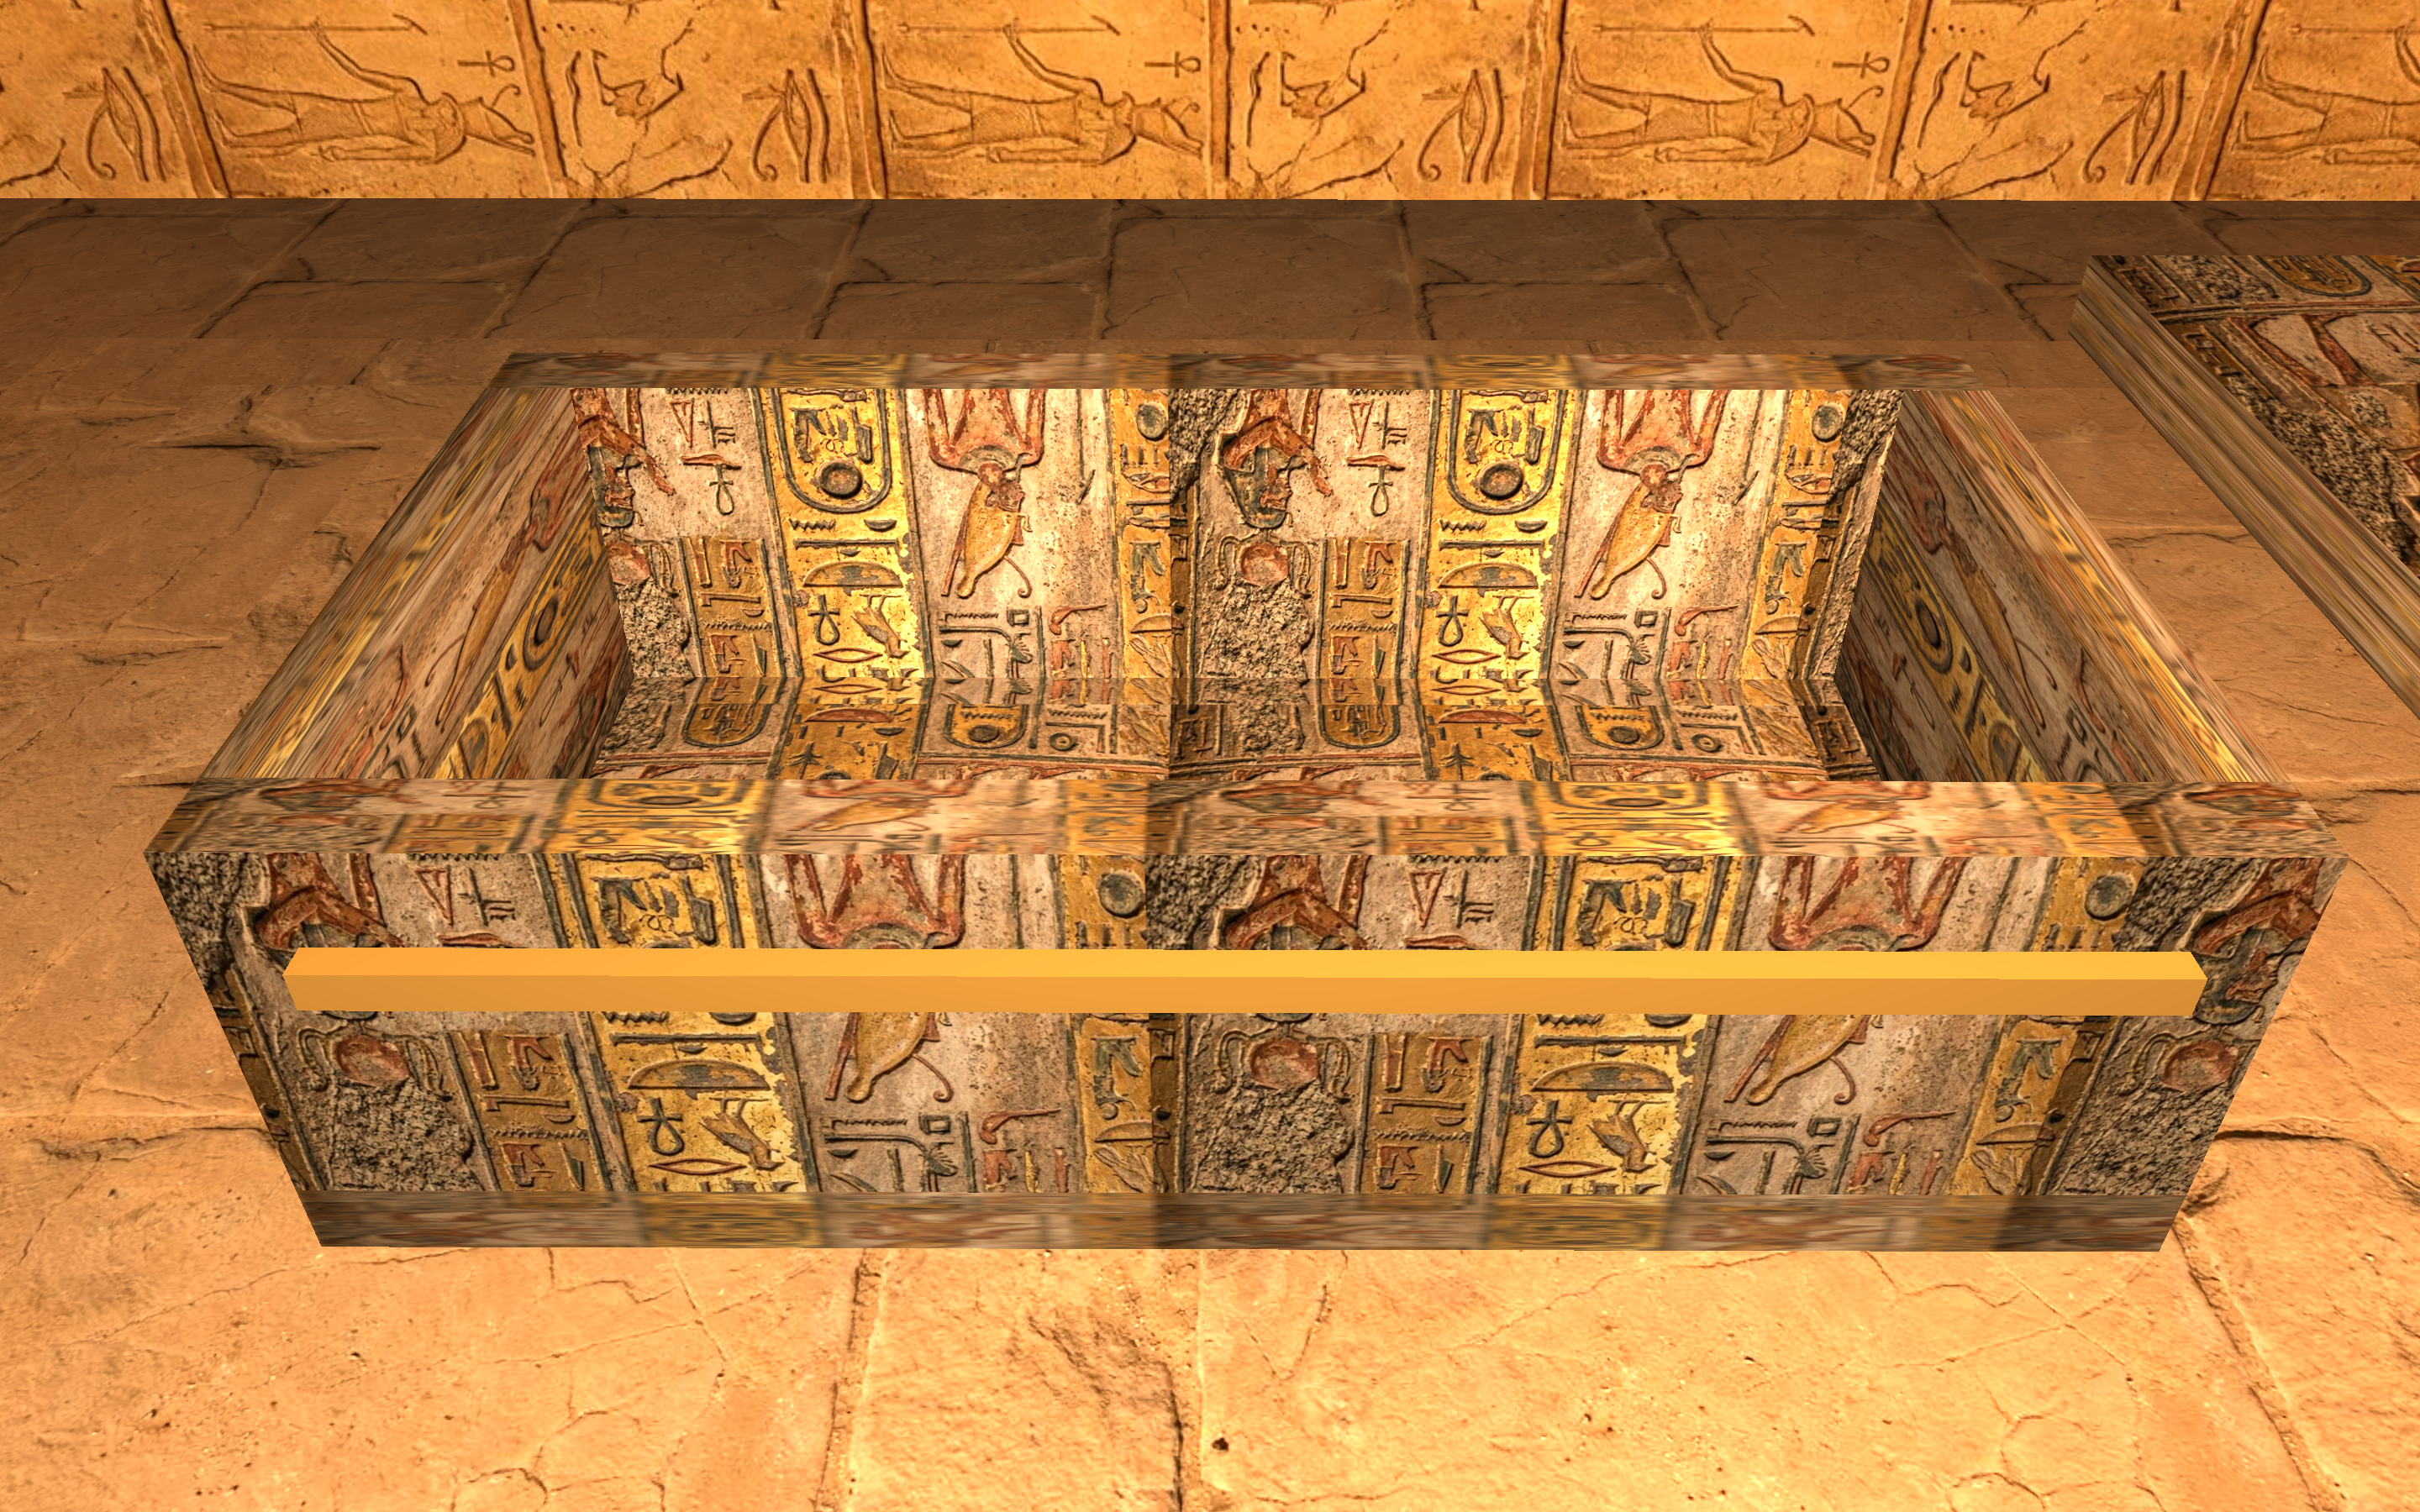
\includegraphics[width=0.9\textwidth]{screenshots/16.png}
    \caption{Interacting with the Sarcophagus triggers continuous uniform interpolation metrics directly smoothly sliding the intricate structural lid model across orthogonal properties revealing internal modeled parameters efficiently without compromising bounds.}
    \label{fig:open_sarcophagus}
\end{figure}

\newpage
% ------------------------- SECTION 5: INTERACTIONS & CONTROLS -------------------------
\section{Interaction Design \& Mechanics}
The simulated environment bridges theory and direct user interaction smoothly traversing immediate configurations toggling matrix execution logic evaluated at runtime parameters correctly.

\subsection{Standard Spatial Navigation}
\begin{itemize}
    \item \textbf{W/A/S/D:} Linear transformation mapping velocity vectors interpolating position points physically tracking bounding coordinates.
    \item \textbf{Mouse Movement:} Recalculates yaw and pitch orientations computing spherical logic to dynamically supply values altering \texttt{glm::lookAt} parameters real-time.
    \item \textbf{Space / Shift:} Manipulates independent global Y-axis velocity simulating flight solely operational outside structural limitations scaling parameters.
\end{itemize}

\subsection{Dynamic Graphics Rendering Overrides}
The native implementation intercepts distinct input signals binding modifications directly to shader uniform mappings rendering execution adjustments efficiently:

\begin{table}[H]
\centering
\begin{tabular}{@{}llp{8cm}@{}}
\toprule
\textbf{Shortcut} & \textbf{Concept Focus} & \textbf{Rendering Result Action} \\ \midrule
\texttt{[ / ]} & Bezier Curve Bounds & Adjusts cubic wave offset amplitudes increasing wave distortion values.\\
\texttt{, / .} & Fractal Algorithms & Alters recursive iterations dynamically recalculating palm tree geometries.\\
\texttt{T} & Texture Operations & Subverts sampling bindings natively exposing primitive wire color models.\\
\texttt{4, 5, 6} & Phong Specifications & Explicitly toggles isolated Ambient, Diffuse, or Specular illumination calculations overriding algorithms.\\
\texttt{8 / 9} & Highlight Shininess & Exponentially alters mathematical gradients widening highlight bounds realistically.\\
\texttt{1, 2, 3} & Source Illumination & Enables global Directional Sunlight calculations, isolated Point Lantern physics, or restrictive Handheld Spotlights.\\
\texttt{0} & Spotlight Angles & Linearly iterates defined threshold radius parameters controlling bounds.\\
\texttt{V} & Dynamic Viewports & Overlaps matrix manipulation splitting buffer buffers spanning Orthographic, Isometric, Top and FPS perspectives concurrently.\\ \bottomrule
\end{tabular}
\caption{Real-time shader rendering execution modification controls.}
\end{table}

\newpage
% ------------------------- SECTION 6: CONCLUSION -------------------------
\section{Final Conclusion \& Future Extensibility}
\textit{The Crypt of Thoth} efficiently translates highly theoretical graphics rendering mathematical bounds into an engaging, cohesive interactive virtual platform. Executing intricate geometric properties involving parametric surface boundaries, fractal algorithms mapping and hierarchical structural layouts natively highlights deep control over foundational rendering APIs independent from exterior simulation systems. The project achieves an immersive visual progression applying advanced Phong illumination components meticulously applying localized lighting properties effectively reacting to independent object configurations mathematically.

\textbf{Extensibility Considerations:} 
Iterating beyond strictly bounds natively opens massive improvements implementing linear depth shadow volume mapping algorithms dynamically computing visual obstructions natively mirroring precise environment elements spanning realistic depths. Proceeding incorporating global ambient occlusion maps would structurally improve primitive rendering boundaries inside narrow tomb geometries significantly augmenting authentic structural representation effectively tracking interactive progression logically.

\end{document}
